
% !TEX root = root.tex
\chapter{Linear and Nonlinear Microrheology of Lysozyme Layers Forming at the Air--Water Interface}
\chaptermark{Lysozyme Layers}

\section{\label{sec:introduction}Introduction}

When an aqueous protein solution forms an interface with air or an oil, the protein molecules can discover the interface through diffusion and adsorb.~\cite{Walder2011}  The adsorption process is commonly believed to include conformational changes to the protein that lift hydrophobic substructures out of the aqueous surroundings. As the interface ages, it becomes increasingly crowded with adsorbed protein, and its rheology changes dramatically.~\cite{Murray2011a}
The mechanical properties of interfacial protein layers are an important aspect of their biological function, as in films that form on lachrymal secretions~\cite{Rosenfeld2013} and saliva~\cite{Proctor2005}, and in their role in biomedical and food processing technologies.~\cite{Murray2002}  In particular, the mechanical behavior of interfacial protein layers can enhance the stability of droplets and bubbles in emulsions and foams.~\cite{SaintJalmes2005,McClements2004}
Protein layers are fragile, molecularly thin, and spatially heterogeneous films whose properties evolve with time. These features complicate traditional interfacial rheometry measurements and often make results difficult to interpret.  Recently, microrheology techniques have shown promise as an alternative method to characterize the evolving mechanical behavior of protein layers.  

The basic approach of microrheology, which is most often employed to study bulk materials, involves tracking the motion of colloids embedded in the material to probe its mechanical properties.  Passive microrheology connects Brownian fluctuations of colloids to a material's linear shear response. Active microrheology infers the drag on colloids driven by an external forcing and relates that drag to mechanical response through a linear or nonlinear model relating stress and strain.
Applying microrheology to an interfacial system like a protein layer presents particular challenges. The theory supporting microrheology assumes Stokes drag, which is subtle in two dimensions.~\cite{Saffman1975} Moreover, colloidal probes at an interface experience drag forces from both the interfacial layer and from the underlying subphase. Since no exact closed-form solution for the drag on a membrane-bound object exists, one must rely on analytical and numerical approximations that apply in various limits.~\cite{Hughes1982,Fischer2006,Sickert2007,Petrov2008,Levine2004a}

Nevertheless, despite these challenges, microrheology has found increasing application in the study of films at fluid-fluid interfaces including not only protein layers~\cite{Lee2009, Lee2010, Lee2011, Dhar2010, Prasad2006} but also polymer layers,~\cite{Helfer2001, Kandar2010, Maestro2011} lipid monolayers,~\cite{Sickert2007, Choi2011, Kim2011, Park2011, Murakami2010} and particle-laden interfaces.~\cite{Wu2009a, Langer2012}  This work has included studies of both the linear shear rheology and nonlinear mechanical response of interfacial films.  Recently, our group investigated the interfacial microrheology of layers of the protein $\beta$-lactoglobulin  at air-water and oil-water interfaces.~\cite{Lee2010, Lee2011}  These experiments included both active and passive microrheology measurements that enabled us to track the transition from viscous to elastic mechanical behavior as the layers form.  In both $\beta$-lactoglobulin adsorbing to the air-water and to an oil-water interface, the microrheology revealed a viscoelastic transition consistent with gel formation.  However, features of the transition, such as the rate of layer formation and degree of spatial heterogeneity, varied strongly between the two cases.~\cite{Lee2010, Lee2011} 

Although the viscoelastic transition in protein layers is often ascribed to network formation through intermolecular association,~\cite{Bos2001, Murray2002, Martin2002, Bantchev2003, Roberts2005, Murray2011a} and indeed the evidence from microrheology for gelation in $\beta$-lactoglobulin layers supports this scenario, other mechanisms for the onset of elasticity in  protein layers, particularly involving glass transitions, have been proposed.~\cite{Wierenga2006, Cicuta2005, Cicuta2003, Cicuta2007}  Therefore, in an effort to understand better those aspects of the viscoelastic transition in protein layers that are universal and those that are system specific, we have conducted a microrheology study of layer formation at the air interface of lysozyme solutions. As described in Section \ref{sec:background} below, layers formed by lysozyme at the air-water interface are good candidates for microrheology investigations.  Our study included passive measurements, which tracked the Brownian motion of spherical colloids at the interface, and active measurements in which the rotational motion of magnetic nanowires at the interface was employed to infer layer rheology.  The experimental methods are described in Section \ref{sec:procedures}.  As described in Section \ref{sec:results}, the passive measurements provide information about the linear frequency-dependent shear modulus of the layers, while the active measurements probe properties of the layer's nonlinear stress response.  Together the measurements track the interfacial rheology as it evolves through a viscoelastic transition with increasing layer age.  We discuss in Section \ref{sec:discussion} two possible frameworks for understanding this mechanical evolution:  gelation and the formation of a soft glass phase.  Finally, Section \ref{sec:conclusion} offers some conclusions from the study.



\section{\label{sec:background}Background}

Lysozyme is a single-chain globular protein comprised of 129 amino acids with molecular dimensions 3.0 $\times$ 3.0 $\times$ 4.5 nm$^3$ and molecular weight 14,300 g/mol.  The molecule is considered a ``hard'' protein that is rigid against conformational fluctuations, due in part to the presence of four internal disulphide bridges.  Correspondingly, lysozyme is stable against denaturation over an unusually large range of bulk solution conditions.  However, it readily adsorbs at the air-water interface, and interfacial rheometry measurements on mature interfacial layers reveal that they can acquire pronounced elasticity.\cite{Roberts2005,Malcolm2006}   The structural properties of adsorbed lysozyme layers have been studied in detail by neutron and x-ray reflectivity.\cite{Lu1998,Lu1999,Yano2009}   In addition, surface-sensitive spectroscopies have interrogated the conformational state of the absorbed molecules.\cite{Postel2003a,Lad2006a}  Interpretation of the reflectivity measurements has led to debate about the structure of adsorbed lysozyme.  While neutron reflectivity results indicate that the lysozyme retains its globular structure with no significant denaturation, time-resolved x-ray reflectivity results indicate that the molecules initially adsorb in a flat, unfolded structure.  Evidence for conformational changes is further provided by Fourier transform infrared spectroscopy, which indicates adsorbed lysozyme contains antiparallel $\beta$-sheets that are absent in the native structure.\cite{Lad2006a}   However, no direct evidence exists for the breaking of the internal disulphide bridges are upon adsorption.  In absorbed layers of other protein species, such as  $\beta$-lactoglobulin, the formation of intermolecular disulphide bridges is seen as an important feature of layer formation.  By characterizing the viscoelastic transition in interfacial lysozyme layers, we seek to correlate properties of the viscoelastic behavior with possible structural models to provide further insight into the layer formation.

As described in the next section, we focus our study on lysozyme solutions with a fixed bulk concentration of 0.05 mg/ml, for which the reflectivity indicates dense monolayers form at the interface.\cite{Lu1998,Lu1999}  Specifically, this concentration is near the upper limit at which the thickness of mature layers, approximately 3.0 nm, is the same as more dilute layers.  At somewhat higher concentrations, the layer thickness increases, indicating a reorientation of the molecules at the interface, presumably due to crowding.  At far higher concentrations, lysozyme can form multi-layers at the air-water interface.  However, those concentrations are two orders of magnitude greater than in the present study.\cite{Lu1998}  Hence, in this study we consider monolayers of protein.


\section{\label{sec:procedures}Experimental Methods}

\subsection{\label{sec:sample_prep}Sample Preparation}

Lyophilized powder of chicken-egg lysozyme (Sigma Aldrich, purity of 98\%) was mixed gently \cite{Stathopulos2004} into 10 mM sodium phosphate buffer, pH 7.4, at room temperature to obtain solutions with 0.05 mg/ml protein. The solutions were employed within minutes of preparation.
For the measurements, samples were contained in a 1-cm inner-diameter cylinder with an inner surface whose bottom half was aluminum and top half was Teflon, so that when solution filled the cell to the appropriate level, the aluminum--Teflon seam pinned the air--water interface, creating a flat surface with no meniscus.
To begin, we filled the cylinder nearly to the seam with 0.5 ml of the protein solution. The age of the sample $t_a$ was measured from the moment the cell was filled with solution, creating a fresh interface with the air.
A spreading solution containing either spherical or nanowire colloids (discussed below) was prepared in advance and sonicated to disperse any colloidal aggregates. In addition to the colloids, the spreading solution contained equal parts buffer solution and isopropanol (IPA).~~To introduce the colloids to the interface, we touched a 10-$\mu$L droplet of the spreading solution to the surface. The solution wet the interface, depositing colloids uniformly over the surface.   Evaporation of the IPA typically caused convective flows at the interface that persisted for about one minute.  All measurements were performed only after these flows ceased.  After each experiment, the sample cell was cleaned thoroughly by scrubbing and sonicating in Alconox soap solution, acetone, and IPA, and then rinsed repeatedly in deionized water.

We note the presence of the IPA in the spreading solution could potentially influence layer formation at the interface.  Measurements of the sample mass over time indicated that some of the IPA evaporated within seconds while the rest mixed into the bulk, where if uniformly distributed it constituted at most 1\% of the solution.  While lysozyme is stable in such dilute IPA solutions at room temperature, the near-surface IPA concentration was likely larger at times shortly after application of the spreading solution, and the protein can denature at IPA concentrations above 20\%.~\cite{Velicelebi1979}  Further, even at concentrations below which the alcohol does not denature the lysozyme, its interactions with the protein could affect the protein's hydrophilicity, which would impact its adsorption properties.  To understand the possible effects of the IPA, we performed additional experiments using pure buffer as the spreading solution and found that the IPA did not significantly affect the interface's subsequent rheological properties.  Because we achieved better surface coverage of colloids by including IPA in the spreading solution, all results discussed here were obtained with this sample preparation. 

\subsection{Passive (Brownian) Microrheology}

For the passive microrheology measurements, we employed charge-stabilized polystyrene spheres (Interfacial Dynamics Corp.)~with radius 0.5~$\mu \text{m}$. We observed the colloids at the interface using an inverted bright-field microscope with a 40X objective (WD 2.7-3.7 mm, NA 0.6). A video camera (Nikon D3100) recorded a 300$\times$170-$\mu$m field of view at a rate of 30 frames per second, which set the shortest time over which probe motion could be characterized. (The exposure time was approximately 0.033 s, the inverse of the frame rate.)  Video was captured continuously, so that, in principle, probe trajectories could be followed for arbitrarily long durations. However, for analysis, the videos were divided into segments whose duration was restricted by the evolving dynamics at the interface during layer formation.

We extracted probe trajectories from the video using a custom Python implementation~\cite{trackpy} of the widely-used Crocker--Grier multiple-particle-tracking algorithm.~\cite{Crocker1996} 
We accounted for static and dynamic errors in the particle tracking, which can qualitatively distort microrheology measurements if left uncorrected.\cite{Savin2005}
Typically between 30 and 200 probes were in view at any time, constituting up to 0.3\% surface coverage. As the experiment proceeded, some probes encountered each other and aggregated, reducing the population of usable probes.  Also, we corrected for drift of the probes at the interface, which was more severe than in a typical bulk microrheology measurement, by subtracting the average velocity of the ensemble from that of each particle.

In general, particle mobility in an interfacial film is affected by drag from both the film and from the adjacent bulk fluid phases.  The bulk contribution is most important when the interfacial viscosity is small, and theories have been developed to separate the contributions.~\cite{Sickert2007, Levine2004, Dhar2006, Fischer2004a, Fischer2006, Levine2004a}  When the interfacial viscosity is large or the layer is viscoelastic, the subphase contribution is less important, and, as described below, the measurements on lysozyme layers were in this regime.  In this case, under appropriate conditions, one can obtain the frequency-dependent interfacial shear modulus $G^*(\omega)$ from the Brownian motion of the probes through a two-dimensional version of a generalized Stokes-Einstein relation,  \cite{Helfer2001, Maestro2011}
\begin{equation}
 G^*(\omega)=\frac{k_B T}{\pi i\omega \mathcal{F}_u \{\langle \Delta r^2 (t) \rangle \} }  \label{eq:StokesEinstein}
\end{equation}
where $\langle \Delta r^2 (t) \rangle$ is the particles' ensemble-average mean-squared displacement and $\mathcal{F}_u \{\langle \Delta r^2 (t) \rangle \}$ is its unilateral Fourier transform.  


\subsection{Active Microrheology}

\subsubsection{Magnetic Nanowire Probes.}~For the active microrheology measurements, we employed ferromagnetic nickel wires, whose fabrication has been described elsewhere.~\cite{Tanase2001} The wires, which had radius $R_w=0.175\ \mu$m and lengths $L$ from 5 to 30 $\mu$m, possessed a large magnetic moment ($\mu/\text{L} = 3\times10^{-14}\text{A}\cdot\text{m}^2/\mu\text{m}$) parallel to their axis. 
The wires were hydrophobically functionalized with n-octadecyltrimethoxysilane (OTMS) and spread onto the interface as described above. The functionalized wires make a contact angle at the air--protein solution interface of $\theta_c = 79\degree \pm 1\degree$, as determined previously,~\cite{Lee2010} implying the wires were approximately half-submerged.

\subsubsection{Microscopy with \textit{in situ} Magnetic Fields.}~Custom-built ``magnetic tweezers'' mounted on an inverted microscope (Nikon TE2000), were employed to apply time-dependent magnetic torques to an isolated wire at the interface.~\cite{Lee2009} The tweezers, consisting of two sets of four solenoids with ferromagnetic cores positioned symmetrically above and below the microscope focal plane, could produce fields in any direction within the focal plane.  A feedback mechanism in the electronics controlling the tweezers created rise times below 2 ms for a step change in the field.  A high-speed camera (Photron Fastcam), recording a 70 $\mu$m $\times$ 70 $\mu$m view at frame rates up to 1000 fps, captured the wire's motion.  The wire's orientation in each video frame was determined by analyzing the gray-scale image and treating the brightness of each pixel as an effective mass to calculate the principal ``inertial axis''.  With this procedure, we could resolve the orientation with an estimated precision of $\pm 0.1\degree$, a tenfold improvement over our previous method.~\cite{Lee2010} 
%With the wires pinned at the interface of the sample, we applied a magnetic torque $\Gamma_\text{mag.} = \vec{\mu} \times \vec{B}$ to rotate the wires in the plane of the interface.
%
%For a viscous interface, the relative contributions from interface and bulk are parameterized by $l_0=\eta_s/\eta$, the ratio of the surface viscosity $\eta_s$ to the bulk viscosity $\eta$. When the wire's length $L \lesssim l_0/10$, the rotational viscous drag $\zeta \approx 1.48L^2\eta_s$ \cite{Levine2004, Levine2004a}.

\subsubsection{Measurement Procedures and Analysis.}~Measurements of layer response to applied magnetic torques on wires were performed in the time domain using step changes in magnetic-field direction of 90\degree.~~Prior to the change in field direction, the field was oriented parallel to the wire, and hence to the wire's magnetic moment. Following the change in field direction, the wires experienced a magnetic torque, 
\begin{equation}
\Gamma_\text{mag} = \mu B \sin{\theta}
\end{equation}
where $\theta$ is the angle between the wire axis and the field, causing the wires to rotate in the plane of the interface.  Each measurement was repeated at several field values to test for linearity.  In most cases, fields between 30 and 50 Gauss were selected since they caused the wires to rotate with angular velocities that were well matched to the video frame rate.  At some later ages, when the layer imposed larger resistance to the wire rotation, field values up to 100 Gauss were employed.   In the low-Reynolds-number conditions of the measurement, the magnetic torque was balanced by the hydrodynamic drag and/or any elastic stresses from the interfacial layer and subphase.  In the case of a simple viscous drag, 
\begin{equation}
  \mu B \sin\theta = \zeta_r \dot{\theta}
  \label{eq:wire_eq_motion}
\end{equation}
\noindent where $\zeta_r$ is the drag coefficient.  The solution to Eq.~(\ref{eq:wire_eq_motion}) gives the resulting time dependence between the field and wire axis,\cite{Sasha} 
\begin{equation}
  \theta(t) = 2 \tan^{-1} \left[ \exp \left( -\frac{\mu B}{\zeta_r} (t-t_0) \right) \right]
  \label{eq:sasha}
\end{equation}
where $t_0$ is an experimental parameter that accounts for uncertainty in the time that the wire begins rotating in response to the field change and can differ from zero by an amount up to the time between video frames.  For such a viscous interface, the relative contributions to the rotational drag from the interface and subphase are parameterized by the Saffman length, $l_0=\eta_s/\eta$, the ratio of the interfacial viscosity $\eta_s$ to the subphase viscosity $\eta$. When the wire's length $L < l_0/10$, the interface dominates the drag, and one finds \cite{Levine2004}

\begin{equation}
  \zeta_r = 1.48 L^2\eta_s
  \label{eq:wire_zeta}
\end{equation}
 
 As described below, in the active microrheology measurements on lysozyme layers, we observed that in some cases the rotational motion of the wires was consistent with simple viscous drag, Eq.~(\ref{eq:sasha}). However, in other cases, particularly at large layer age, we observed deviations from Eq.~(\ref{eq:sasha}) that we identify as a consequence of a nonlinear response by the layer to the stress imposed by the rotating wire.  Specifically, we find in these cases that the layer's response is well described as that of a non-Newtonian, power-law fluid. A power-law fluid is characterized by the stress-strain relation
\begin{equation}
\sigma = K\dot{\gamma}^{n}
\label{eq:pf}
\end{equation}
\noindent where $\sigma$ is the stress, $\dot{\gamma}$ is the strain rate, $K$ is known as the consistency, and the exponent $n$ is known as the flow index.  When $n=1$, Eq.~(\ref{eq:pf}) reverts to the stress-strain relation of a viscous liquid, while $n < 1$ and $n > 1$ correspond to shear-thinning and shear-thickening behavior, respectively. More generally, power-law fluids are a special case of Herschel-Bulkley fluids, which are characterized by a power-law stress-strain relationship above a yield stress, $\sigma_0$,
\begin{equation}
\sigma = \sigma_0 + K\dot{\gamma}^n
\label{eq:HB}
\end{equation}
\noindent Such non-Newtonian response is observed in a wide range of soft disordered materials including paints, plastics, polymeric solutions, and food products.~\cite{Alexandrou2001a}

Adopting a power-law fluid response like Eq.~(\ref{eq:pf}) to describe the wire motion under the influence of a magnetic torque leads to
\begin{equation}
  \mu B \sin\theta = (\zeta_{\text{pl}} \dot{\theta})^n.
  \label{eq:pf_wire}
\end{equation}
\noindent where the nonlinear drag coefficient $\zeta_{\text{pl}}$ has dimensions $(\text{N}\cdot\text{m})^{1/n}\cdot\text{s}$. An analytical solution to Eq.~(\ref{eq:pf_wire}) for $\theta(t)$ is not available; however, the inverse function $t(\theta)$ is:
\begin{align}
\label{eq:pf-solution}
  t(\theta) =&\left[\frac{\zeta_{\text{pl}}}{(\mu B)^{1/n}}\frac{n}{1-n}\right]\times\\ \notag
      &\sin^{1 - 1/n}\theta\ _2\text{F}_1\left(\frac{1}{2}, \frac{n-1}{2n}, \frac{3n-1}{2n}; \sin^2 \theta\right)\bigg\vert^{\theta}_{\pi/2} - t_0
\end{align}
\noindent where $_2\text{F}_1$ is the ordinary hypergeometric function and $t_0$ is the same small experimental parameter introduced in Eq.~(\ref{eq:sasha}).  As described below, we employ this form with $n < 1$ to analyze the wire rotation in the lysozyme layers.  However, we emphasize that Eq.~(\ref{eq:pf_wire}) should only approximate the torque relation in a power-law fluid.  A more precise relation would need to account fully for the flow generated in the layer around the wire, and specifically for its spatially varying shear gradients, and would not lend itself to straightforward comparison with experimental results.  Nevertheless, as shown below, Eqs.~(\ref{eq:pf_wire}) and (\ref{eq:pf-solution}) accurately capture the rotational motion of wires in lysozyme layers, indicating a nonlinear response characteristic of a power-law fluid.  


\section{\label{sec:results}Results}

\subsection{\label{sec:linear}Linear Rheology}

The rheology at an air interface with the lysozyme solutions evolves quickly following the formation of the interface, with viscoelastic behavior emerging within minutes in the passive measurements, consistent with reflectivity studies that indicate lysozyme adsorbs rapidly at the air-water interface.\cite{Yano2009}  Figure~\ref{fig:emsds} shows examples of the ensemble-averaged mean-squared displacement $\langle \Delta r^2(t) \rangle$ of the colloidal probes at a several ages $t_a$ since creation of the interface.  For reference,  the mean-squared displacement of colloids at the air interface of pure buffer containing no protein is also shown.  In the absence of adsorbing protein, $\langle \Delta r^2(t) \rangle$ varies linearly with lag time indicating simple viscous drag with a viscosity consistent with water.  At the interface of the protein solution, the mobility of the probes evolves rapidly at early layer ages; therefore, $\langle \Delta r^2(t) \rangle$ at each age is determined based on video segments of limited duration (less than one minute).  For this reason, the maximum lag time $t$ is restricted to $ t \leq 1$ s to assure adequate statistics.  Within the resulting limited dynamic range, $\langle \Delta r^2(t) \rangle$ is well described as a power law, $\langle \Delta r^2(t) \rangle \sim t^{\alpha}$. As shown in Fig.~\ref{fig:power-law_expon}, the power-law exponent $\alpha$ steadily decreases with increasing age, signifying increasingly subdiffusive particle motion. Following analysis based on the generalized Stokes-Einstein relation, Eq.~(\ref{eq:StokesEinstein}), power-law behavior in the mean-squared displacements of the colloidal probes, $\langle \Delta r^2(t) \rangle \sim t^{\alpha}$ with $\alpha < 1$, implies the lysozyme layer's linear shear modulus, $G^*(\omega) = G'(\omega) + iG''(\omega)$, has power-law frequency dependence, $G'(\omega) \sim G''(\omega) \sim \omega^{\alpha}$.~\cite{Mason2000}  The significance of this power-law frequency dependence and its evolution with layer age is discussed in Section \ref{sec:discussion} below.


\begin{figure}
 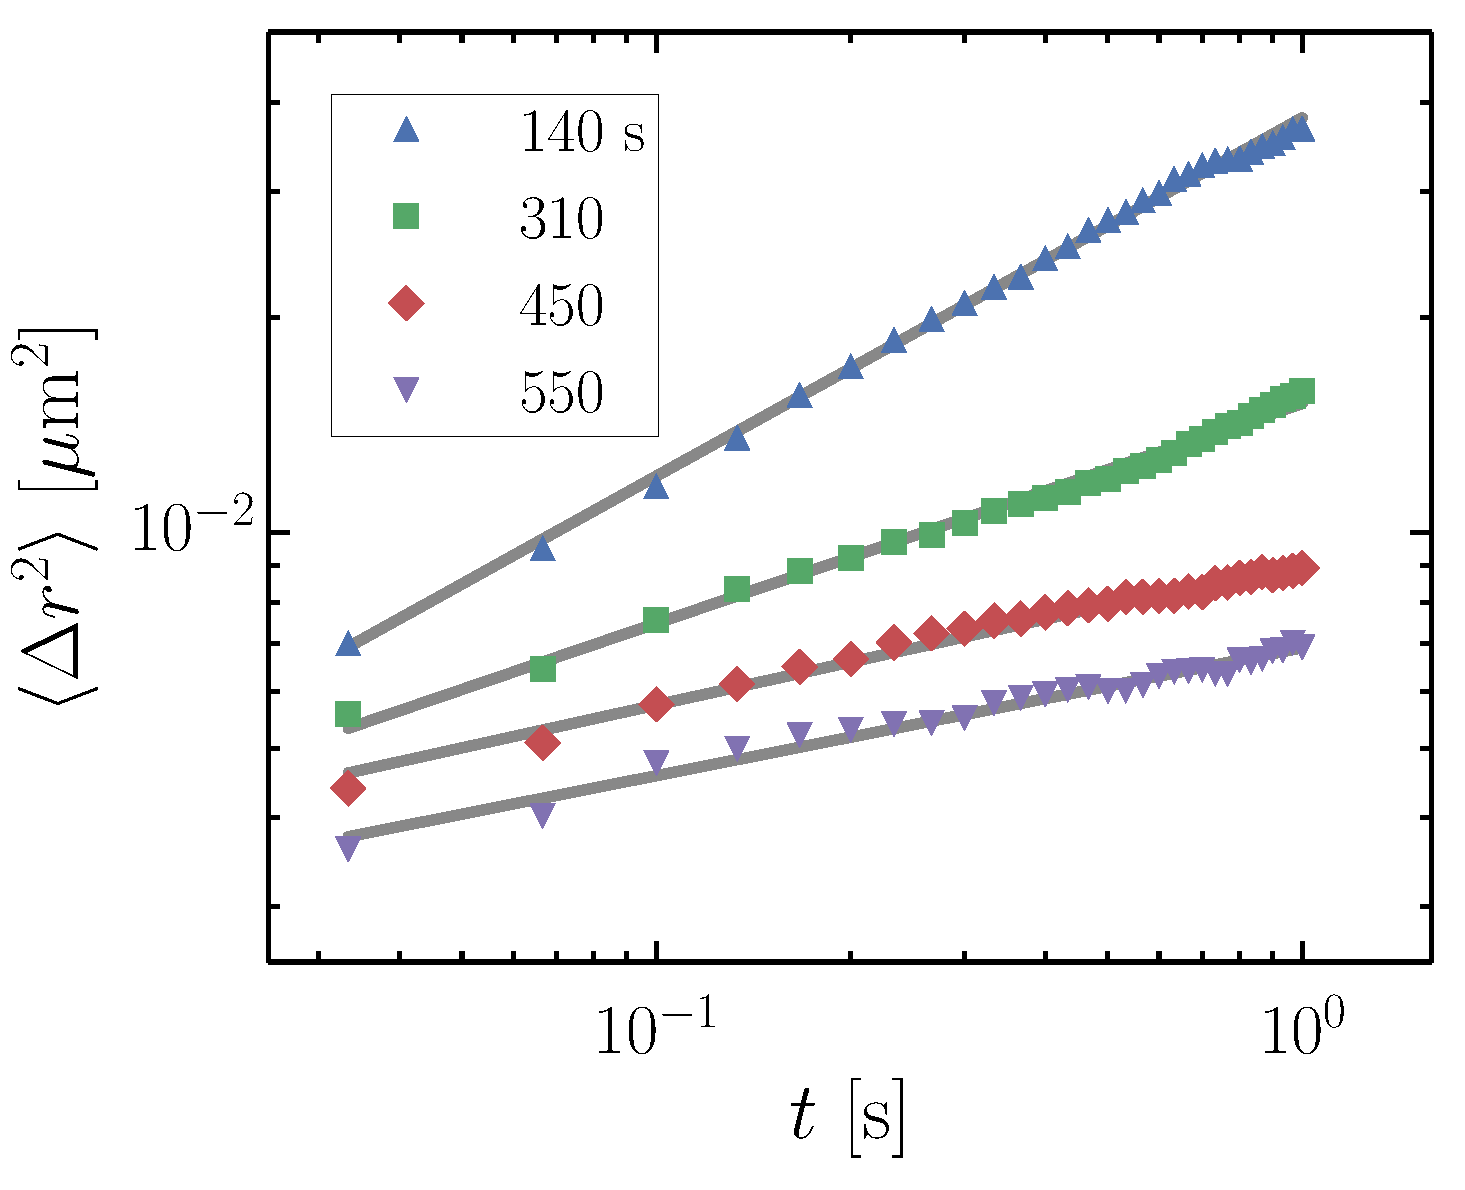
\includegraphics[width=\linewidth,keepaspectratio]{lysozyme/Fig1_msd}
 \caption[\lofimage{lysozyme/Fig1_msd}Ensemble-average mean-squared displacements of colloids at the air interface]{\label{fig:emsds}Ensemble-average mean-squared displacements of 0.5-$\mu$m radius colloids at the air interface of a lysozyme solution (0.05 mg/ml, pH 7.4) at ages $t_a$ = 140 (squares), 310 (diamonds), 450 (triangles), and 550 (solid circles) seconds since formation of the interface.  Also shown is the mean-squared displacement of the probes at the air-buffer interface in the absence of protein.  The solid lines are the results of power-law fits.}
\end{figure}


\begin{figure}
 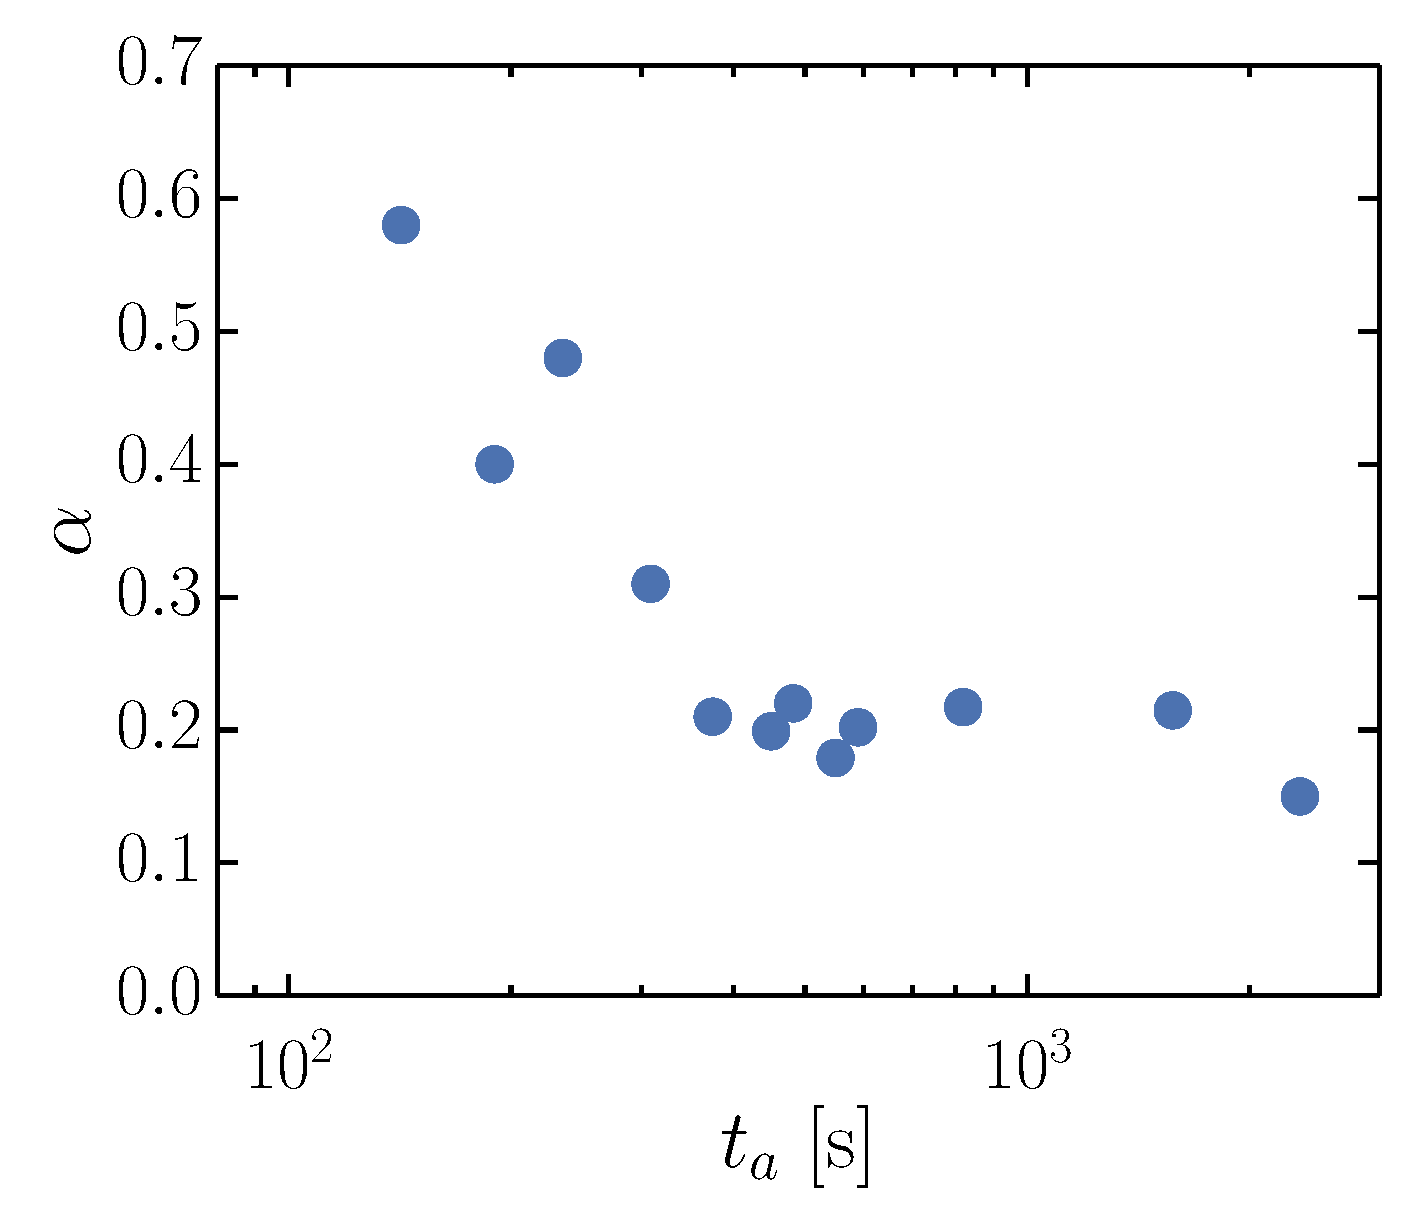
\includegraphics[width=\linewidth,keepaspectratio]{lysozyme/Fig2_power-law-exponent}
 \caption[\lofimage{lysozyme/Fig2_power-law-exponent}Power-law exponent characterizing $\langle \Delta r^2(t) \rangle \propto t^{\alpha}$ as a function of age]{\label{fig:power-law_expon} Power-law exponent characterizing the ensemble average mean-squared displacements, $\langle \Delta r^2(t) \rangle \propto t^{\alpha}$, of colloids at the air interface of a lysozyme solution as a function of the age since formation of the interface.}
\end{figure}

%Such weak power-law frequency dependence is characteristic of the shear rheology of a broad range of complex fluids including concentrated microgel solutions \cite{ketz}, foams \cite{khan}, paint \cite{mackley}, intracellular matrix [Ref], compressed emulsions \cite{mason_colloid},  particulate suspensions, slurries, and liquid-crystal nanocomposites [RanjiniPRL]. In these cases, the power-law exponent typically lies in the range $\alpha \approx$ 0.1 to 0.3.  The soft glassy rheology model~\cite{sollich}, which explains this response as a general consequence of structural disorder and metastability, provides a unifying theoretical framework for this behavior.  In this model, $$ serves as an effective noise temperature, with systems approaching a glass transition as $n \rightarrow 0$.  Thus, the steady decrease in $n$ with layer age seen in Fig.~\ref{fig:power-law_expon} points to increasingly glassy dynamics characterizing the structural response of the lysozyme layer.  Ultimately, at very late ages $\langle \Delta r^2(t) \rangle$ becomes independent of lag time $t$, as illustrated by the results at $t_a$ = ??? minutes in Fig.~\ref{fig:emsds}.  That is, ultimately at very late ages $n \approx 0$.  Thus, such mature lysozyme layers can be considered soft glasses.

%A noteworthy feature of the evolution in probe mobility is the nearly immediate influence of the protein adsorption on the interfacial rheology, as revealed by the onset of subdiffusive behavior, $n \approx 0.6$, less than 3 minutes after layer formation.  This rapid impact of adsorption of lysozyme on the interface  contrasts strongly with layer formation at the air-water interface  of $\beta$-lactoglobulin solutions of similar concentration [LeeLangmuir].  $\beta$-lactoglobulin layers forming at the air-water interface  remain viscous for a protracted period during which the interfacial viscosity increases slowly and undergo a  transition to elastic behavior only at ages of tens of minutes.  This viscoelastic transition is further characterized by pronounced mesoscale heterogeneity in colloidal mobility, where some colloids become localized as if trapped in an elastic film while others continue to undergo diffusion as if in a viscous environment [LeeLangmuir].  We observe no such pronounced heterogeneity in probe mobility at the interface of the lysozyme solutions.  Rather, all probes undergo statistically similar evolution in mobility represented by the ensemble averages in Fig.~\ref{fig:emsds}.  

%The rapid evolution in $\langle \Delta r^2(t) \rangle$ seen in Fig.~\ref{fig:emsds} is more similar to that observed at the oil-water interface of $\beta$-lactoglobulin solutions, where again the onset viscoelastic behavior occurs at a new interface within minutes and no pronounced mesoscale heterogeneity is observed [LeeSoftMatter].  However, more detailed comparison of $\langle \Delta r^2(t) \rangle$ at those interfaces and in the lysozyme layers reveal important differences.  Specifically, evolution in probe mobility in $\beta$-lactoglobulin layers indicated the layers underwent a quasi-two dimensional gel transition, with $\langle \Delta r^2(t) \rangle$ showing characteristics of critical stress relaxation.  In contrast, as mentioned above, we identify the evolving shear rheology of the entry of the layers into a soft glass phase.  We note Cicuta et al. similarly identified layers of $\beta$-lactoglobulin spread on the air-water interface as soft glassy materials [Cicuta].  These different experiments on $\beta$-lactoglobulin and lysozyme together hence indicate that the evolution in the rheology of interfacial protein layers is not universal, and depending on  specific conditions -- such as protein species, hydrophobic phase (e.g., air or oil), and how the protein is introduce onto the interface -- either gel and or glass transitions can underlie the observed viscoelastic transitions.



\subsection{\label{sec:nonlinear}Nonlinear Rheology}

As in the passive microrheology, the active nanowire microrheology reveals a pronounced evolution in the mechanical behavior of the lysozyme layers with increasing layer age.  Close inspection of the results in the active measurements and comparison with those from the passive measurements, however, show that they probe a different aspect of the layer response, specifically its nonlinear rheology.  For example, Figs.~\ref{fig:early-and-late-rotation}(a) and \ref{fig:early-and-late-rotation}(b) display the angle $\theta$ between an 11-$\mu$m-long wire and an applied magnetic field as a function of time following a 90\degree\ step change in the direction of the field at layer ages $t_{\text{a}}=$ 2700 s and 8200 s, respectively.  At early ages, such as $t_{\text{a}}=$ 2700 s (Fig.~\ref{fig:early-and-late-rotation}(a)), the wire rotates rapidly in response to the magnetic torque so that the angle between the wire axis and the magnetic field relaxes fully to zero in a short time, and the response at these ages is consistent with the wire experiencing simple viscous drag.  The dashed line through the data in Fig.~\ref{fig:early-and-late-rotation}(a) shows the result of a fit using the form for viscous drag, Eq.~(\ref{eq:sasha}), which agrees closely with the data.  Such agreement is observed at all layer ages up to $t_a \approx 3000$ seconds.  The interfacial viscosity extracted from the fit using Eq.~(\ref{eq:wire_zeta}) is 21 nPa$\cdot$m$\cdot$s, which implies $L\eta/\eta_s \approx 2$, near the lower limit of interfacial viscosity where Eq.~(\ref{eq:wire_zeta}) is a valid approximation for the drag coefficient. 

\begin{figure}
  \centerline{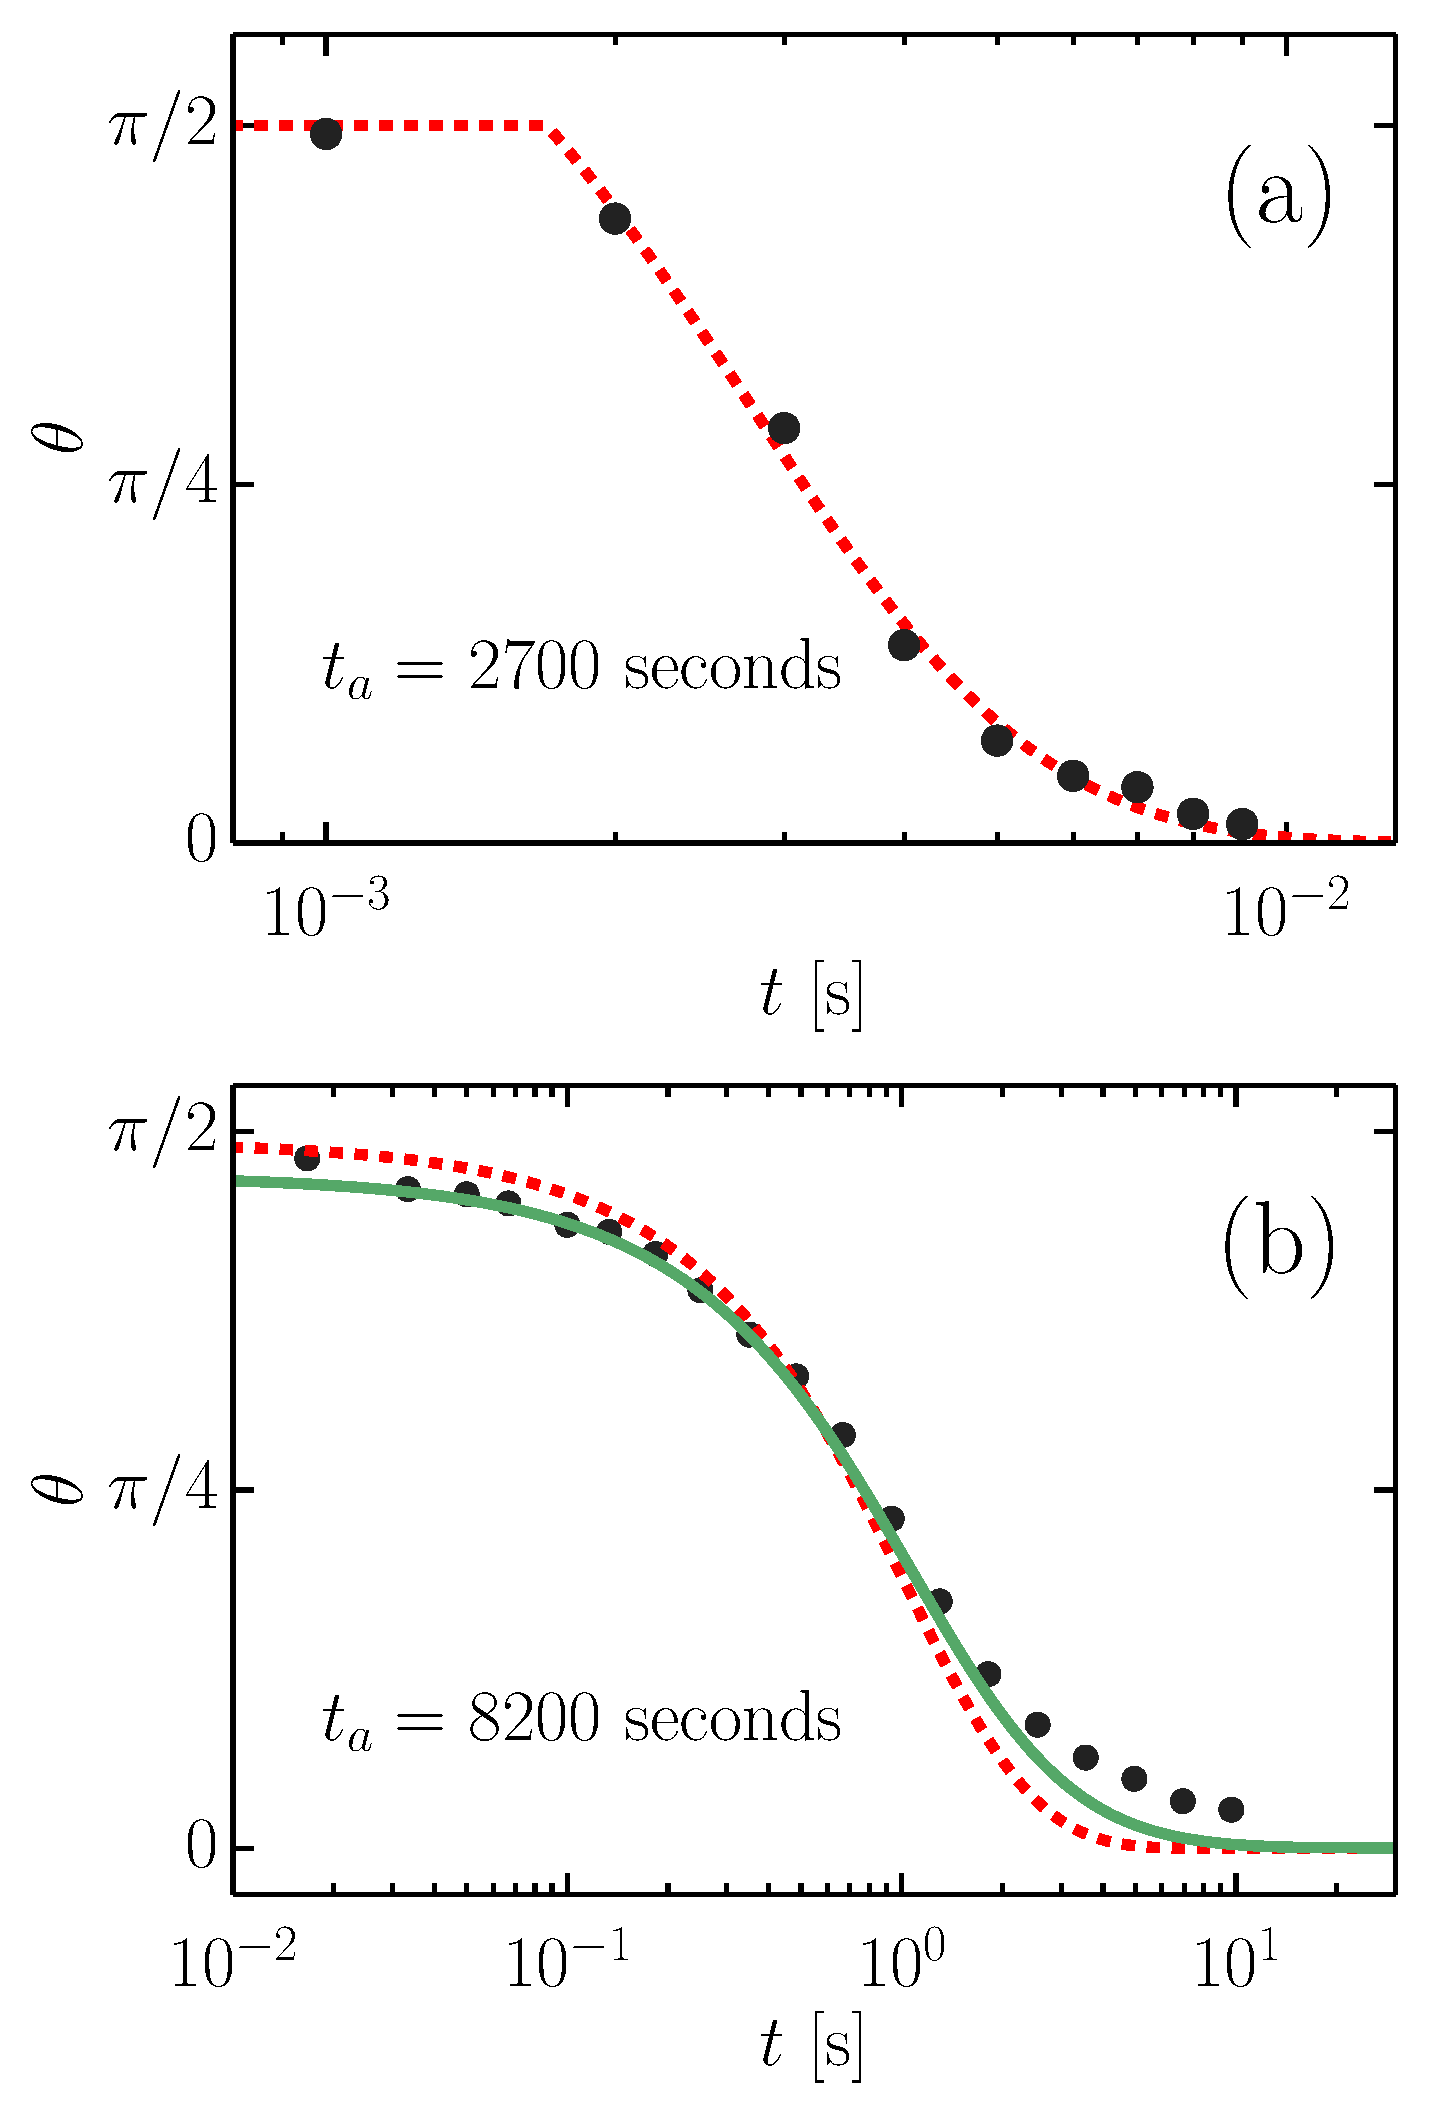
\includegraphics[width=\linewidth,height=0.8\textheight,keepaspectratio]{lysozyme/Fig3_compare-early-late}}
 \caption{\label{fig:early-and-late-rotation} Angle between the axis of a 11-$\mu$m-long Ni nanowire and external magnetic field as a function of time following a step change in the field direction of 90\degree~at interface ages (a) $t_{\text{a}}=$ 2700 s ($B = 30$ G) and (b) $t_{\text{a}}=$ 8200 s ($B = 60$ G).  The dashed lines in (a) and (b) are the results of fits to the data using a form based on simple viscous drag (Eq.~(\ref{eq:sasha})), and the solid line in (b) is the result of a fit using a form based on drag from a power-law fluid (Eq.~(\ref{eq:pf-solution})).}
\end{figure}

Notably, this value of interfacial viscosity, 21 nPa$\cdot$m$\cdot$s, is the same order as that measured previously on $\beta$-lactoglobulin layers at early ages~\cite{Lee2010}.  However, as described in Section~\ref{sec:linear} above, during this span of early ages where the active measurements appear consistent with a viscous layer, the passive measurements show increasingly viscoelastic behavior.  This apparent discrepancy results from the active measurements accessing a nonlinear rheological response from the layers.  Hence, one should not interpret this result as the linear, zero-shear-rate viscosity of the lysozyme layers.  The nonlinear nature of the response is shown clearly in analysis of the nanowire rotation at later ages when the shape of $\theta(t)$ becomes no longer consistent with simple viscous drag.  This change is illustrated by the dashed line in Fig.~\ref{fig:early-and-late-rotation}(b), which shows the result of a fit using Eq.~(\ref{eq:sasha}) to the data at $t_a = 8200$ s and which reveals pronounced deviations of $\theta(t)$ from the viscous lineshape.  Such systematic deviations are apparent in the angular response of the wire at all ages greater than 3000 s.  The solid line through the data in Fig.~\ref{fig:early-and-late-rotation}(b) depicts the result of a fit using the power-law-fluid form, Eq.~(\ref{eq:pf-solution}), to the data with $n \approx 0.6$.  As the fit illustrates, good agreement between the data and Eq.~(\ref{eq:pf-solution}) is found for all ages.  That is, for $t_{\text{a}} < $ 3000 s, best fits with Eq.~(\ref{eq:pf-solution}) give $n \approx 1$ and are indistinguishable from fits with Eq.~(\ref{eq:sasha}), while at later ages $n < 1$, implying shear-thinning behavior.  We note that for shear-thinning power-law fluids, the apparent zero-shear-rate viscosity $\eta_{app}\equiv \sigma/\dot{\gamma} \sim \sigma^{1-1/n}$ diverges in the limit of small shear stress, consistent with the nearly elastic response observed in the passive microrheology at ages greater than 3000 s.

%We note the introduction of the flow index $m$ gives Eq.~(\ref{eq:pf-solution}) one additional free parameter over Eq.~(\ref{eq:sasha}). (QUESTION:  WHAT PARAMETER IN EQ. (7) PLAYS THE ROLE OF $t_0$?)  To provide an alternative comparison between the nonlinear behavior implied by Eq.~(\ref{eq:pf-solution}) and linear viscoelastic behavior, we also include in Fig.~\ref{fig:early-and-late-rotation}(b) the result of a fit of a Maxwell model~\cite{Wilhelm2003} to the data at $t_a = 137$ minutes, shown by the dotted-dashed line. While the inclusion of an elastic component in the layer response improves the agreement over that of strictly viscous drag, the quality of the fit with the Maxwell model is inferior to that with the power-law-fluid model. Thus, the success of Eq.~(\ref{eq:pf-solution}) implies that the nanowire motion probes the nonlinear rheology of the layer.  

While Eq.~(\ref{eq:pf-solution}) describes accurately the angular rotation of the wire through the protein layer, the nonlinear nature of the hypergeometric function makes obtaining stable values for $n$ and $\zeta_{\text{pl}}$ through fits using Eq.~(\ref{eq:pf-solution}) problematic.  However, an alternative approach to modeling the power-law-fluid response is obtained by rearranging the torque balance relation, Eq.~(\ref{eq:pf_wire}), to get
\begin{equation}
\label{eq:pf_linearized}
  \ln(\dot{\theta})= \frac{1}{n}\ln(\sin\theta) + \ln\left(\frac{(\mu B)^{1/n}}{\zeta_{\text{pl}}}\right)
\end{equation}
\noindent Thus, the power-law-fluid model predicts that the logarithm of the time derivative of $\theta(t)$ varies linearly with the logarithm of $\sin\left(\theta\right)$ and that the inverse of the flow index $1/n$ is the proportionality constant.  As a test of this prediction, Fig.~\ref{fig:linearization} shows results for the wire rotation at a series of layer ages plotted in this way, where the values of $\ln(\dot{\theta})$ are obtained from $\theta(t)$ through the Savitzky-Golay smoothing algorithm.~\cite{Savitzky1964}  As the figure indicates, the data follow a linear relationship as expected from Eq.~(\ref{eq:pf_linearized}).~~Further, we find that linear fits with Eq.~(\ref{eq:pf_linearized}) provide a more reliable method of obtaining $n$ than do direct fits to $\theta(t)$ using Eq.~(\ref{eq:pf-solution}).~~For instance, the change from $n \approx 1$ at early ages to shear-thinning behavior at late ages is seen clearly in the change in slope of the data in Fig.~\ref{fig:linearization}.  Figure \ref{fig:m-with-age} displays the values of $n$ extracted from fits using Eq.~(\ref{eq:pf_linearized}) as a function of layer age.  The flow index appears to undergo an abrupt decrease around $t_{\text{a}} = $ 3000 s from $n \approx 1$ to $n \approx 0.7$.  (The data could also be interpreted as a steady decrease in $n$, but one should not expect that $n$ extrapolates at early times to values greater than one, which would imply shear-thickening behavior.)  The values of $n$ obtained for the lysozyme layers at late ages are typical of shear-thinning materials that behave as power-law fluids, where in most cases $0.3 < n < 1$ is observed.~\cite{Huang1998a, Larrard1998}   

\begin{figure}
  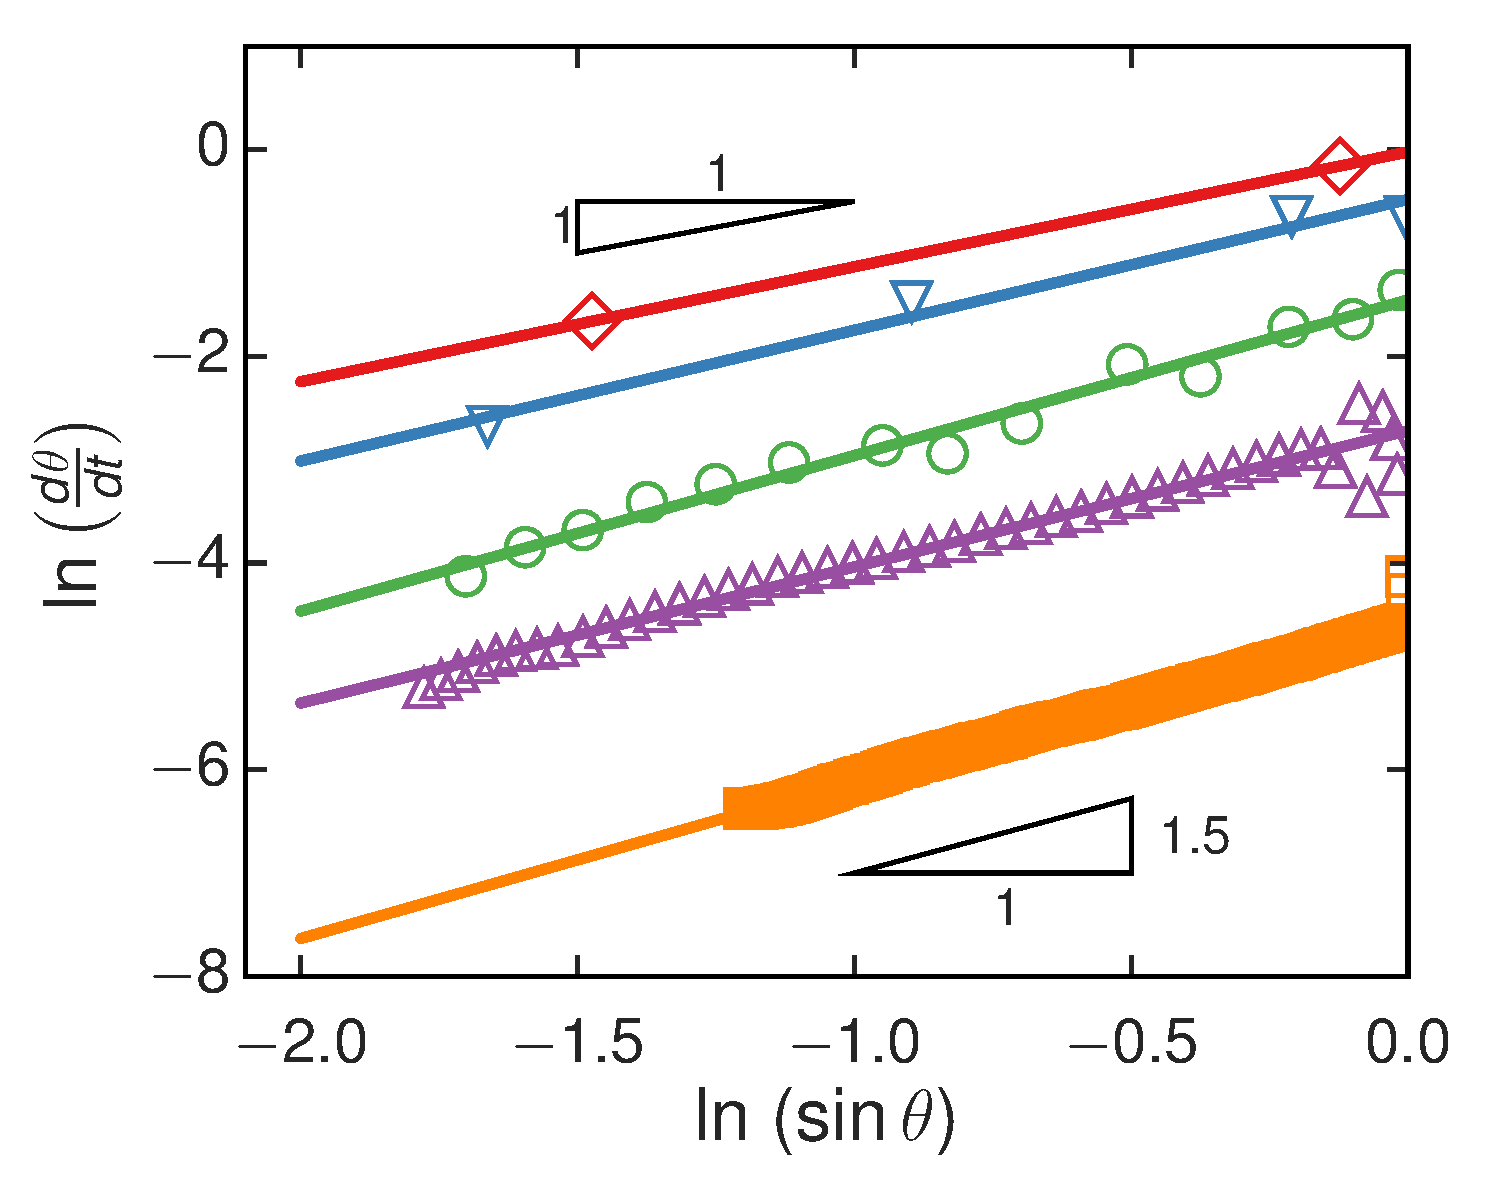
\includegraphics[width=\linewidth,keepaspectratio]{lysozyme/Fig4_linearization-AT20-40G}
 \caption{\label{fig:linearization}  Logarithm of the nanowire rotation rate as a function of the logarithm of $\sin(\theta)$, where $\theta$ is the angle between the wire axis and external magnetic field, at interface ages $t_a =$ 1320 seconds (red circles), 2700 seconds (blue triangles), 3600 seconds (green squares), 5100 seconds (purple diamonds), and 6600 seconds (orange inverted triangles).  The solid lines are the results of linear fits. The slope increases with layer age from near one at early ages to above 1.5 at late ages.}
\end{figure}

%The values of $n$ obtained for the lysozyme layers are typical of shear-thinning materials that behave as power-law fluds, where in most cases $0.3 < n < 1$ is observed [Huang1998a, Larrard1998].  
%Notably, the soft glassy rheology model, which as described above predicts weak power-law frequency dependence in the linear shear modulus $G^*(\omega)$ in disordered soft materials, also predicts power-law fluid behavior in the nonlinear rheology of these materials.  Further, according to the model the flow index increases on approaching the glass transition.  Thus, qualitatively the linear and nonlinear responses of the lysozyme layers fit well together as those of a soft glassy material that approaches a glass phase with increasing age.  [Footnote here noting that according to SGR power-law-fluid $n$ is equal to $n$ from MSD fit, which we don't see, but does anybody?]. 


\begin{figure}
  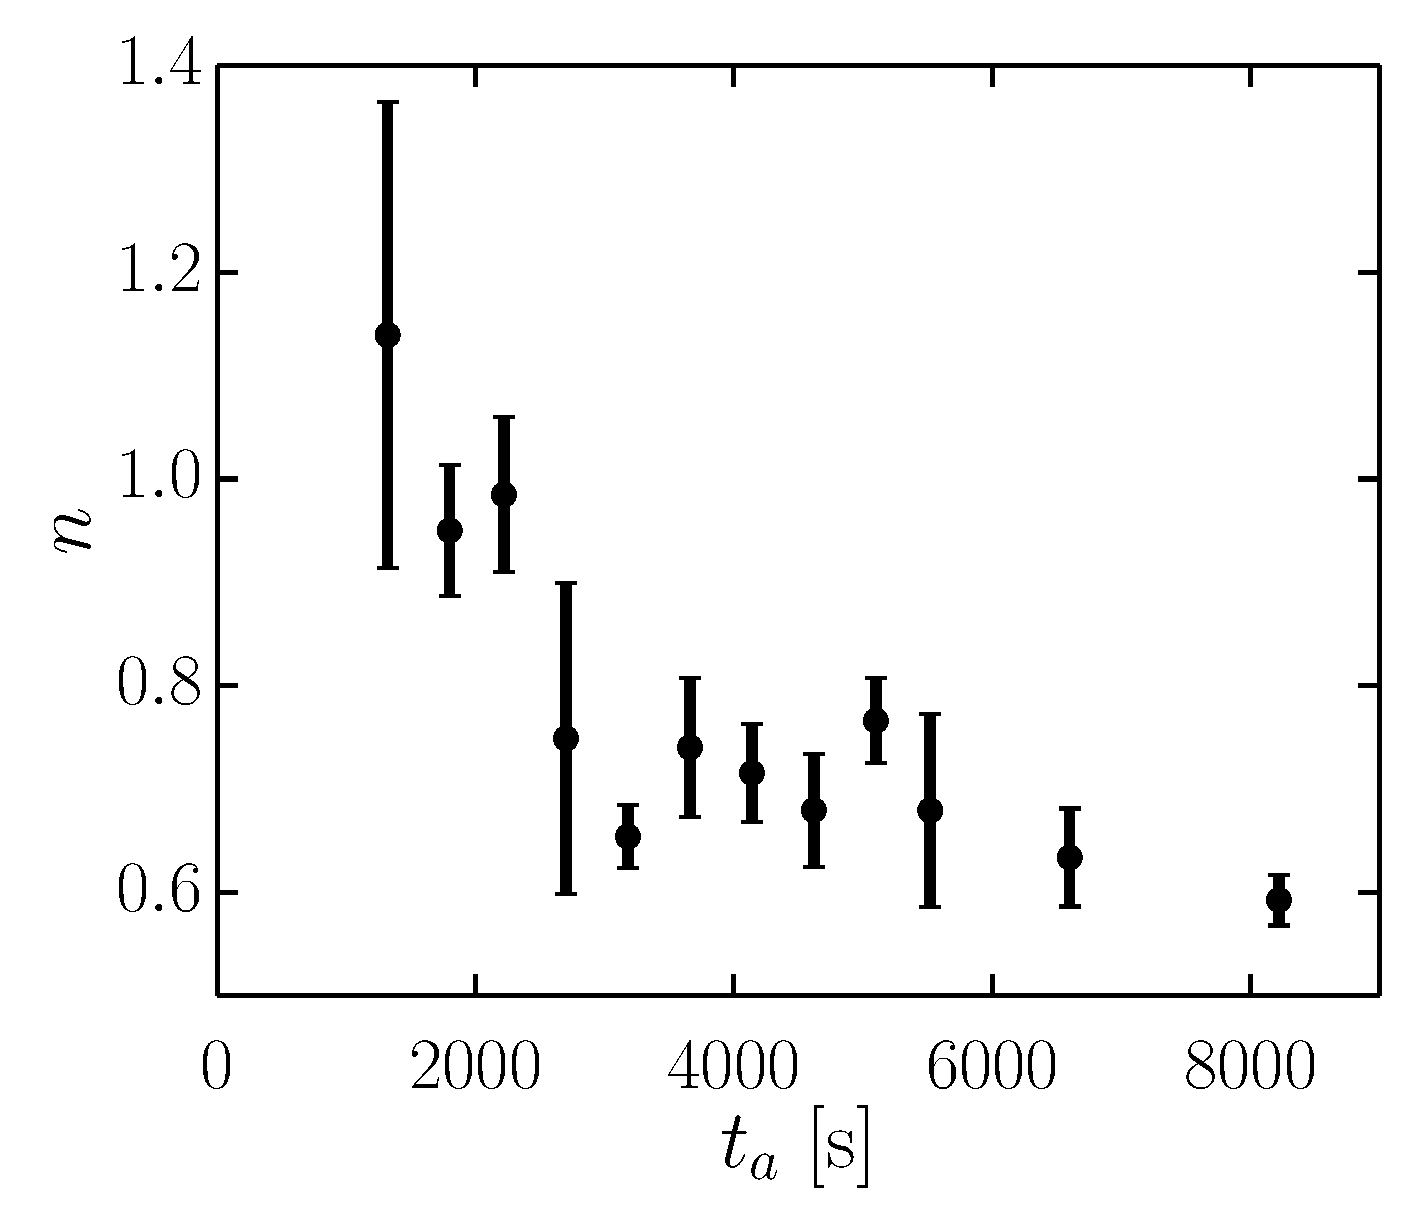
\includegraphics[width=\linewidth,keepaspectratio]{lysozyme/Fig5_m-with-age-avg-fields}
  \caption{\label{fig:m-with-age}Flow index $n$ as a function of layer age. At each age, $n$ is determined from measurements at several magnetic-field values. The error bars incorporate both statistical variation in $n$ and measurement uncertainty.}
\end{figure}


%Applying the re-parameterization to a trial with known purely viscous behavior returned the desired parameter m = 1, and the intercept b was found to decrease with age, as shown in Fig.~(\ref{fig:linearized-AT32}). These results are consistent with an increasing viscosity, though the technical limitations of both the Savitzky-Golay smoothing at sharp derivatives and the logrithmic convolution at shallow derivates prevents accurate extraction of $\zeta_{\text{pl}}$ beyond an order of magnitude. However, extraction of m values through re-parameterization was found to be both robust and reproducable, and ranged from 1 in viscous cases to ~3 for late age samples, consistant with results from direct fitting to the power-law model (Figure here of late age AT20 and AT21).

%The main utility of linear reparameterization is to verify the non-newtonian, power-law behavior of the interfacial layer, and to provide an accurate value of m for use in direct fitting of the analytical solution. 

\begin{figure}
 \centerline{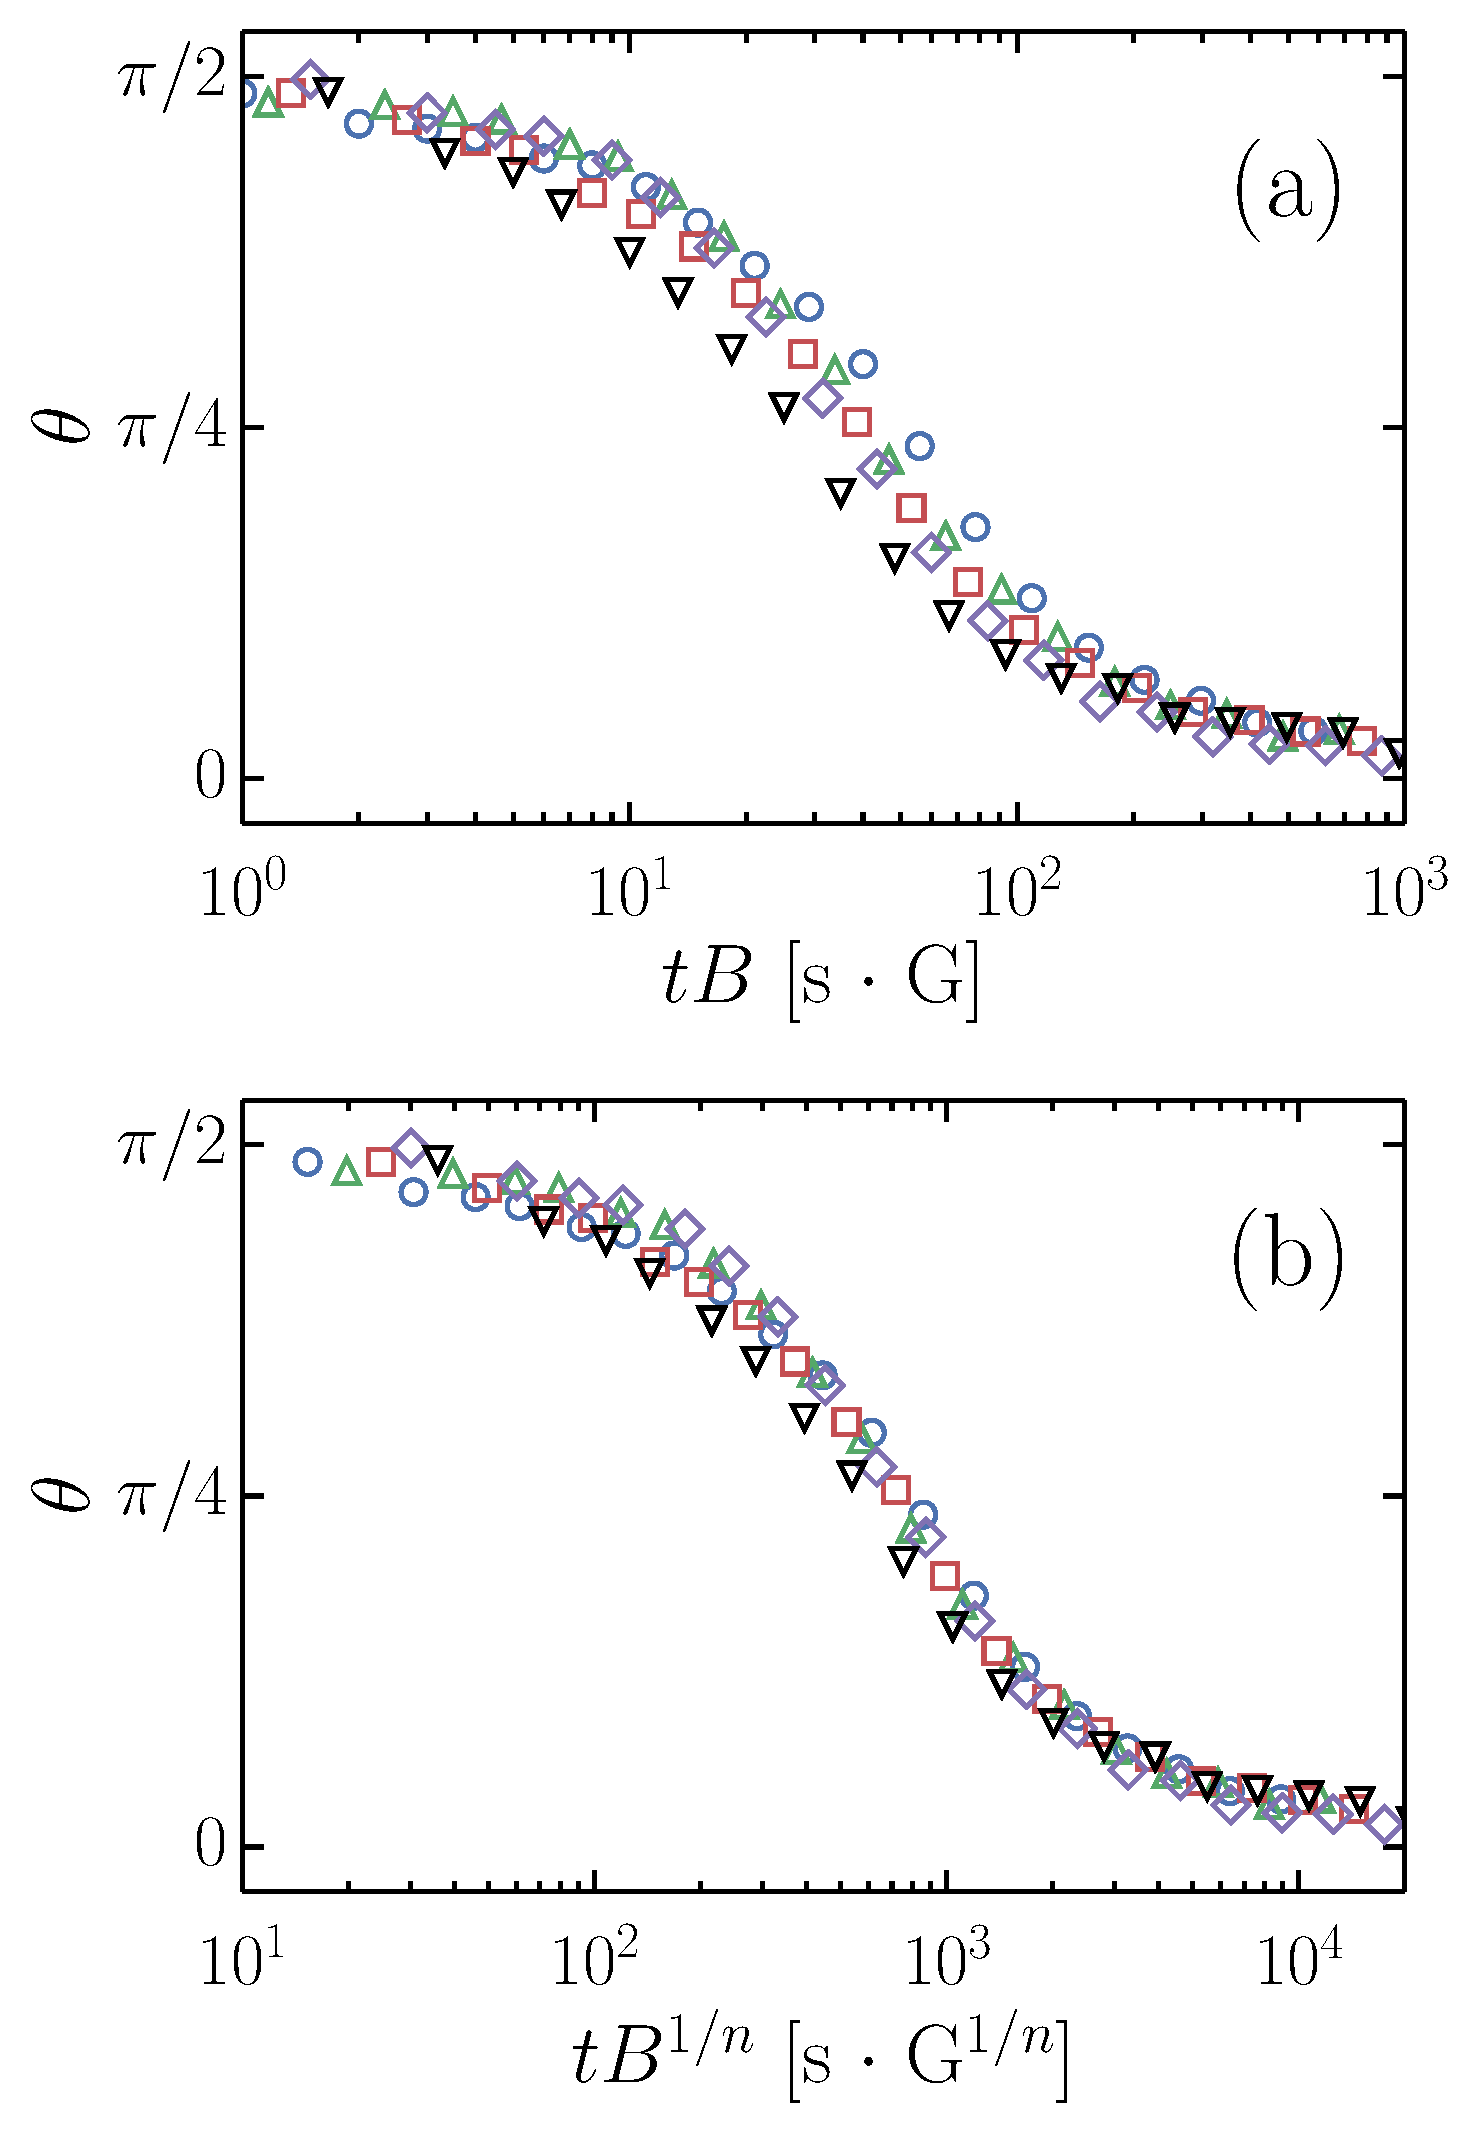
\includegraphics[width=\linewidth,height=0.8\textheight,keepaspectratio]{lysozyme/Fig6_rescaled-curves-137}}
 \caption{\label{fig:scaling}Angle between wire and magnetic field as a function of time scaled by magnetic field strength $B$ for field strengths of 60 (circle), 70 (triangle), 80 (square), 90 (diamond), and 100 G (inverted triangle).  In (a) time is scaled linearly with field strength; in (b) time is scaled by $B^{1/n}$ with $n=0.6$, the value obtained from fits to $\theta(t)$. The interface age is $t_a = 8200$ seconds.}
\end{figure}

While the success of Eqs.~(\ref{eq:pf-solution}) and (\ref{eq:pf_linearized}) provides strong evidence that the layer response in the active microrheology experiments reflects the nonlinear rheology, this nonlinear behavior is more directly demonstrated in the dependence of the wire rotation rate on the magnetic-field strength $B$.  Since the torque on the wire is proportional to $B$, a viscous-like linear response from the layer should lead to a rotation rate that is similarly proportional to $B$.  Figure \ref{fig:scaling}(a) shows results for the rotation angle from a set of measurements at $t_a = 8200$ s at various field strengths with time scaled by $B$.  In contrast to the expectations of linear response, the curves at different $B$ fail to collapse.  Better scaling is achieved assuming the nonlinear relation between rotation rate and $B$ implied by the power-law-fluid form of Eq.~(\ref{eq:pf_wire}), as shown in Fig.~\ref{fig:scaling}(b).

A common property of the rheology of shear-thinning, thixotropic materials is a recovery period following application of a nonlinear stress during which the shear-altered structure relaxes back to its quiescent state.  We searched for such effects in the active microrheology on the lysozyme layers by varying the waiting time between wire rotations and by varying the sequence of magnetic field values.   We found no discernible transient behavior for waiting times as small as 2 seconds, the minimum we could access experimentally.

Another key feature of the protein-layer response in the active microrheology is the steady evolution of the timescale of the response as the layer ages.  This evolution is characterized by the dependence of the power-law drag coefficient $\zeta_{pl}$ on layer age, as shown in Fig.~\ref{fig:zeta-powerlaw}.  Because the dimensionality of $\zeta_{pl}$ depends in $n$, for consistency Fig.~\ref{fig:zeta-powerlaw} shows values obtained by fitting $\theta(t)$ at different ages using Eq.~(\ref{eq:pf-solution}) with the flow index fixed at $n=0.70$, its average at ages $t_a > 3000$ s.  As Fig.~\ref{fig:zeta-powerlaw} indicates, $\zeta_{pl}$ grows approximately exponentially, implying a dramatic slowing of the layer response with increasing age. This trend is insensitive to the precise value of $n$ used to obtain $\zeta_{pl}$.  This quasi-exponential increase in the drag is very similar to the behavior seen in earlier studies employing nanowires in active microrheology of protein layers formed from $\beta$-lactoglobulin and albumin.~\cite{Lee2010, Dhar2010}  In those earlier studies, the angular motion was analyzed using a form equivalent to Eq.~(\ref{eq:sasha}), thus assuming a simple viscous response.  However, even in those cases, evidence suggested the nanowire microrheology was accessing nonlinear properties of the layer rheology.~\cite{Lee2010}  Here, the nonlinear nature of the response is seen clearly in the values of the flow index $n$ at late ages and in the nonlinear scaling in Fig.~\ref{fig:scaling}(b).  We note that we repeated the active microrheology measurements on lysozyme layers several times and found that, while an evolution to shear thinning like that depicted in Fig.~\ref{fig:m-with-age} was reproducible, the precise values of $n$ at late ages varied between trials, and we observed instances of layer formation in which the response remained essentially viscous-like ($n \approx 1$), with a viscosity that rose dramatically with age much like $\zeta_{pl}$ in Fig.~\ref{fig:zeta-powerlaw}. While we do not have a firm explanation for this variation in $n$ between trials, we believe these observations support the conclusion that the response shown by the lysozyme layers and those reported previously for $\beta$-lactoglobulin and albumin share the same basic features of nonlinear behavior characteristic of power-law fluids.  


\begin{figure}
  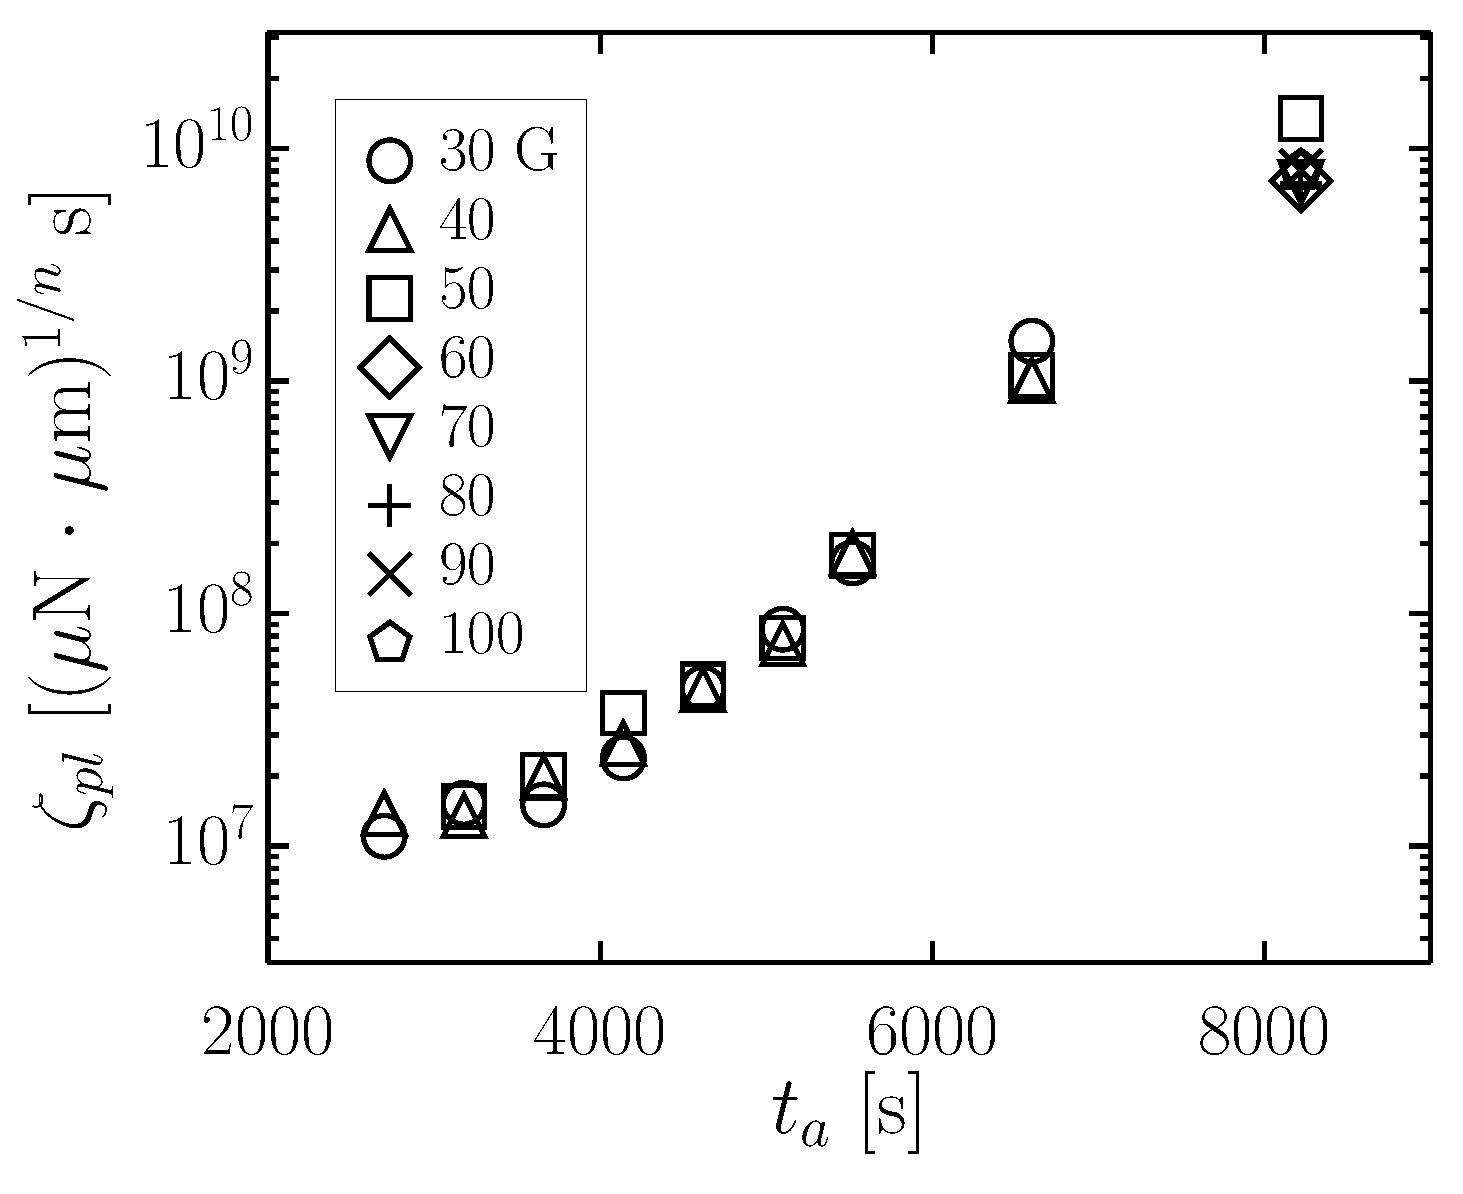
\includegraphics[width=\linewidth,keepaspectratio]{lysozyme/Fig7_zeta-powerlaw}
  \caption{\label{fig:zeta-powerlaw}Power-law drag coefficient $\zeta_{pl}$ as a function of interface age. Values are obtained at a range of field strengths as indicated in the legend and are determined from fits using Eq.~(\ref{eq:pf-solution}) with the flow index fixed at $n = 0.70$, the average value at ages $t_a > 3000$ s.}
\end{figure}

%(Linear reparameterization of the form given in Eq.~(\ref{eq:pf_linearized}) was also applied to films that displayed known Maxwell like viscoelasticity, and a characteristic upward curvature was found in the limit $ln\left(sin\left(\beta - \theta\right)\right)\rightarrow{0}$. This characteristic feature of a Maxwell film was not observed in any trial on lysozyme films.)

%We note the power-law fluid behavior in the nonlinear response persists to very late ages ($t_a > 120$ minutes), when the passive microrheology shows a constant $\langle r^(t) \rangle$ implying an elastic layer with frequeny-indepenent shear modulus.  As mentioned above, within the soft glassy rheology model, this elasticity implies the layer has become a soft glass.  The model further predicts that materials inth  glass phase behave as Herschel–-Bulkley fluids, with a power-law fluid response to stress above a critical yield stress as in Eq.~(\ref{eq:HB}).~~Therefore, an interesting question about the layers' non-Newtonian rheology at very late ages is whether it is precisely that of a power-law fluid or whether the layers possess some small yield stress.  Evidence opposing the existence of any yield stress comes from the linear dependence of $\ln(\dot{\theta})$ on $\ln(\sin\theta)$ in Fig.~\ref{fig:linearization}. The presence of a yield stress would lead to upward curvature on such plots.  Fitting the results at late age using a Hershel-Bulkley form, we can place an upper bound on the yield stress of ???.  In addition, the wires display no measurable recoil when the external field is removed, indicating no stored elastic deformation.   However, as noted above we also observed some variability in the layer response in the active microrheology, both for different trials and for different wires within a single layer, and in some cases wire motion became imperceptible at very late layer ages, and we are unable to distinguish this immobility as the onset of rigidly and or as extremely large $\zeta_{pl}$.  
%Further, additional experiments probing layer formation at the air interface of lysozyme solutions with very low bulk protein concentrations (below 0.01 mg/ml) suggested the adsorb protein associates to form a rigid network.  At these low concentrations, which are inadequate to provide full coverage of the interface through adsorption, we observed wires to rotating off-center, as if partially trapped in an rigid ``island'' of protein.  
%Another property predicted by the soft glassy rheology model for the glass phase is nonergodicity and aging behavior.  One interpretation for the growth in $\zeta_{pl}$ in Fig.~\ref{fig:zeta-powerlaw} is that it reflects physical aging.  However, we believe the growth in $\zeta_{pl}$ stems from other factors.  Aging is usually manifest as a power-law growth in relaxation times with age, not the much stronger exponential growth seen in $\zeta_{pl}$.  A number of changes to the layer such as growing protein concentration, slowly changing protein conformations, and protein-protein association could underlie the growth in $\zeta_{pl}$.

%To understand better the nature of the non-Newtonian response of the layer to the rotating wire, we performed experiments to image the flow field around a wire by spreading spherical colloids and wires together at an interface of a lysozyme solution. After allowing an interfacial layer to form ($t_a$ = 140 minutes), we applied a rotating 100 G field to spin the wires at an angular frequency of 0.5 Hz.  Colloids in the vicinity of each wire served as tracers of the resulting flow around the wire, following circular trajectories as illustrated in Fig.~\ref{fig:wire-flow-field}, which shows an image of spheres along with their trajectories in the vicinity of ?? $\mu$m wire.  Figure~\ref{fig:tangential-velocity} displays the tangential velocity $v$ of the spheres as a function of their radial distance $r$ from the center of the wire.  The velocity decreases approximately inversely with distance, $v \sim 1/r$.  Such $1/r$ dependence is a character of two-dimensional Stokes flow around a rotating body.  Thus, surprisingly, the shear thinning does not measurably alter the flow profile.  (Is this really surprising?  DAN: What was $m$ at the time this measurement was made??  If $m \approx 1$ maybe we should remove this paragraph.)



%\begin{figure}
 %\includegraphics[width=\linewidth,keepaspectratio][\linewidth,keepaspectratio]{graphics/rising-viscosity-AT32}
% \caption{\label{fig:linearized-AT32}In this trial, a 0.1 mg/ml protein solution remained purely viscous in the region observed, with a viscosity that rose steadily with age, indicating increased $\zeta_{\text{pl}}$. Viscosities were extracted using fits to the form Eq.~(\ref{eq:sasha})}
%\end{figure}

%\begin{figure}
%  \includegraphics[width=\linewidth,keepaspectratio][\linewidth, keepaspectratio]{graphics/wire-flow-field}
%  \caption{\label{fig:wire-flow-field}Colored lines trace the trajectories of passive colloidal spheres in the vicinity of a rotating wire.}
%\end{figure}

%\begin{figure}
%  \includegraphics[width=\linewidth,keepaspectratio][\linewidth, keepaspectratio]{graphics/tangential-velocity}
%  \caption{\label{fig:tangential-velocity}The tangential velocity $v$ of colloids varied with their distance $r$ from the center of the wire rotating at 100 Hz. The line is a best fit to power-law, which gives the dependence $v \propto 1/r^{1.08}$}
%\end{figure}

\section{\label{sec:discussion}Discussion}

\subsection{Nature of the Viscoelastic Transition}

The linear and nonlinear rheology of lysozyme layers revealed by the passive and active microrheology, respectively, provide a coherent picture of the layers' viscoelastic transition.  In this section, we discuss two frameworks in which to interpret this transition:  the formation of a soft glass phase and critical behavior associated with gelation.  These two frameworks, while not entirely mutually exclusive, imply different possible microscopic mechanisms driving the viscoelasticity.  As discussed in Section \ref{sec:background} above, reflectivity and spectroscopy studies of lysozyme layers have led to a debate about the degree that lysozyme unfolds upon adsorption.  Since the intermolecular interactions at the interface will depend on conformation, understanding the microscopic origin of the viscoelastic behavior of the layers can potentially contribute to this debate.  As discussed below, both frameworks are successful in accounting for some but not all aspects of the observed evolution in shear rheology.  

\subsubsection{Soft Glassy Rheology Model}~Weak power-law frequency dependence of $G^*(\omega)$, like that implied by the power-law growth in $\langle \Delta r^2(t) \rangle$, is characteristic of the rheology of a broad range of disordered complex fluids including concentrated microgel solutions,~\cite{Ketz1988} foams,~\cite{Khan1988} paint,~\cite{Mackley1994} intracellular matrix,~\cite{Fabry2001} compressed emulsions,~\cite{Mason1995}  clay suspensions,~\cite{Bonn2002} and liquid-crystal nanocomposites. \cite{Bandyopadhyay2005}   In most cases, the power-law exponent typically lies in the range $\alpha \approx$ 0.1 to 0.3.  The soft glassy rheology model,\cite{Sollich1998} which explains this response as a general consequence of structural disorder and metastability, provides a unifying theoretical framework for this behavior.  Cicuta {\it et al.} have identified layers of $\beta$-lactoglobulin spread on the air-water interface as such soft glassy materials.\cite{Cicuta2003}  Significantly, no specific interparticle associations are required to form soft glassy phases, and purely repulsive interactions within a crowded interface would be sufficient.  Thus, the picture of lysozyme layers as soft glasses is consistent with the protein retaining its native conformation upon adsorption.  In the model, $\alpha$ serves as an effective noise temperature, with systems approaching a glass transition as $\alpha \rightarrow 0$.  Thus, within this picture the steady decrease in $\alpha$ with layer age seen in Fig.~\ref{fig:power-law_expon} points to increasingly glassy dynamics characterizing the structural response of the lysozyme layers.  Notably, the soft glassy rhoelogy model also predicts power-law fluid behavior in the nonlinear rheology of these materials.  Further, according to the model the flow index decreases on approaching the glass transition.  Thus, the linear and nonlinear responses of the lysozyme layers qualitatively fit well together as those of a soft glassy material that approaches a glass phase with increasing age.  More quantitatively, however, the soft glassy rheology model predicts a specific relation between the linear rheology and power-law fluid response,  $n = \alpha$.  The lysozyme layers violate this relation.  This violation suggests that, while the model captures many essential features of the observed mechanical response of the layers, the relationship between structural relaxation and flow in the disordered layers is perhaps more complicated than is assumed in the model.

\subsubsection{Critical Behavior of Gelation}~Materials exhibiting critical stress relaxation on approaching a gel point similarly display weak power-law frequency dependence of $G^*(\omega)$.\cite{Winter1986}  Technically, power-law behavior over an arbitrarily extended range occurs only at the critical point, and at low frequencies (large lag times) the rheology crosses over from viscous-like to elastic as the gel formation progresses.\cite{Winter1986,Veerman2006}  Nevertheless, over a limited dynamic range like that in the passive microrheology measurements, this behavior can appear as a quasi-power law in the mean-squared displacement, $\langle \Delta r^2(t) \rangle \sim t^{\alpha}$, with a power-law exponent that decreases steadily with age.   Indeed, the age-dependent $\langle \Delta r^2(t) \rangle$ in Fig.~\ref{fig:emsds} appear strikingly similar to those obtained in microrheology studies of bulk peptide and polymer solutions undergoing three-dimensional critical gelation.\cite{Veerman2006,Larsen2008}  Identifying the viscoelastic transition in the lysozyme layers with gel formation implies intermolecular bonding capable of creating a percolating network.  The stability of native lysozyme against aggregation in bulk solution suggests that such bonding would require significant unfolding to proceed.  However, anecdotal evidence indicating the adsorbed protein indeed associates to form a network comes from additional active microrheology experiments at the air interface of lysozyme solutions with very low bulk protein concentrations (below 0.01 mg/ml).  At these low concentrations, which are inadequate to provide full coverage of the interface through adsorption, we observed wires to rotate off-center, as if partially trapped in an ``island'' of protein that would form only through attractive interactions.  

\subsubsection{Possibility of a Yield Stress at Late Ages}~An interesting question is whether the lysozyme layers at very late ages display a yield stress in the microrheology measurements.  According to the soft glassy rheology model, the soft glass phase has elastic linear rheology, $\alpha = 0$, and a nonlinear response characteristic of a Herschel-Bulkley fluid as in Eq.~(\ref{eq:HB}).   Similarly, a gel phase would display a yield stress.  While a decrease in $\alpha$ with layer age like that in Fig.~\ref{fig:power-law_expon} was reproducible in the passive microrheology experiments, the final value of $\alpha$ varied from trial to trial, and in some cases the data at late ages was consistent with $\alpha \approx 0$.  Similarly, we also observed some variability in the layer response in the active microrheology, both for different trials and for different wires within a single layer (which we attributed to heterogeneity in the layers), and in some cases wire motion in response to the magnetic torque became imperceptible at late layer ages.  However, we were unable to distinguish this immobility as the onset of rigidity and or as an extremely large $\zeta_{pl}$, and in no cases could we say for certain that the lysozyme layers acquired a yield stress.  For example, evidence opposing the existence of any yield stress comes from the linear dependence of $\ln(\dot{\theta})$ on $\ln(\sin\theta)$ in Fig.~\ref{fig:linearization}. The presence of a yield stress would lead to upward curvature on such plots.  Fitting to the data at late age using a Hershel-Bulkley form gives a result consistent with zero yield stress and allows us to place an upper bound on the yield stress of $\sim 5 \mu$N/m.  In addition, wires in layers at late age rotated fully through $\pi/2$ (when they turned at all) and displayed no measurable recoil when the external field was removed, indicating no stored elastic deformation.   

%Another property predicted by the soft glassy rheology model for the glass phase is nonergodicity and physical aging.  One interpretation for the growth in $\zeta_{pl}$ in Fig.~\ref{fig:zeta-powerlaw} is that it reflects physical aging.  However, we believe this growth in $\zeta_{pl}$ stems primarily from other factors.  First, physical aging is usually manifest as a power-law growth in relaxation times with age, in contrast to the much stronger exponential growth seen in $\zeta_{pl}$.  Also, a number of other possible changes in the layer with age -- such as growing protein concentration, slowly changing protein conformations, and protein-protein association -- could influence the evolution in rheology and underlie the growth in $\zeta_{pl}$.

\subsection{Comparison with Other Protein Layers}

A noteworthy feature of the evolution in probe mobility in the passive measurements is the nearly immediate influence of the protein adsorption on the interfacial rheology, as revealed by the onset of subdiffusive behavior, $\alpha \approx 0.6$, less than 200 seconds after interface formation.  This rapid impact of adsorption of lysozyme on the interface  contrasts strongly with layer formation seen at the air-water interface  of $\beta$-lactoglobulin solutions of similar concentration.~\cite{Lee2010}  $\beta$-lactoglobulin layers forming at the air-water interface  remain viscous for a protracted period during which the interfacial viscosity increases slowly and undergo a  transition to elastic behavior only at ages of tens of minutes.  This viscoelastic transition is further characterized by pronounced mesoscale heterogeneity in colloidal mobility, where some colloids become localized as if trapped in an elastic film while others continue to undergo diffusion as if in a viscous environment.~\cite{Lee2010}  We observe no such pronounced heterogeneity in probe mobility at the interface of the lysozyme solutions.  Rather, all probes undergo statistically similar evolution in mobility represented by the ensemble averages in Fig.~\ref{fig:emsds}.  The rapid evolution in $\langle \Delta r^2(t) \rangle$ seen in Fig.~\ref{fig:emsds} is more similar to that observed at the oil-water interface of $\beta$-lactoglobulin solutions, where again the onset viscoelastic behavior occurs at a new interface within minutes and no pronounced mesoscale heterogeneity is observed.~\cite{Lee2011}  
%However, more detailed comparison of $\langle \Delta r^2(t) \rangle$ at those interfaces and in the lysozyme layers reveals important differences.  Specifically, the evolution in probe mobility in the $\beta$-lactoglobulin layers at the oil-water interface indicated the layers underwent a quasi-two dimensional gel transition, with $\langle \Delta r^2(t) \rangle$ showing characteristics of critical stress relaxation.  In contrast, as described above, we identify the evolving shear rheology of the lysozyme layers with the entry of the layers into a soft glass phase.  
These different experiments on $\beta$-lactoglobulin and lysozyme taken together hence indicate that the evolution in the rheology of interfacial protein layers is not universal, and that depending on  specific conditions---such as protein species, hydrophobic phase (air or oil), and how the protein is introduce onto the interface--- the viscoelastic transitions can proceed through different scenarios.  

\section{\label{sec:conclusion}Conclusion}

In summary, these microrheology experiments tracking the evolution of the air-water interface during lysozyme adsorption have elucidated the linear and nonlinear properties of the viscoelastic transition that the interfacial protein layer undergoes.  As discussed above, interpreting the nature of this transition can contribute to our understanding of the dominant molecular-scale interactions involved in protein-layer formation.  In our analysis of the viscoelasticity of the lysozyme layers, we considered two frameworks for interpretation:  gelation and the formation to a soft glassy phase.  Further microrheology studies that can distinguish more conclusively between these possibilities would be valuable.   Indeed, a key challenge in the field of disordered soft materials is to correlate microstructural properties with the broad distribution of slow relaxation times that give rise to their characteristic rheology.  The quasi-two-dimensional geometry of the layers lends itself to experimental approaches that are unavailable in bulk systems.  For example, experiments comparing imaging with surface pressure have provided insight into layer formation,\cite{Erickson2000} and correlating the results of such experiments with microrheology could provide important new information.  However, another clear conclusion from the microrheology is the sensitivity of the viscoelastic properties of the layers to the specific conditions under which the proteins encounter and associate with the interface.  Hence, any studies comparing rheology with surface structure, surface pressure, other properties would need to take particular care to achieve identical conditions for valid comparisons.

%\section{Appendix}

%We can simplify $_2\text{F}_1(a, b, c; z)$ by exploiting the simple relationship between arguments $b$ and $c$. In general

%\begin{equation}
%  _2\text{F}_1(a, b, c; z) = 
%  \sum\limits_{k=0}^\infty\frac{(a)_k (b)_k}{(c)_k}\frac{z^k}{k!}
%  \ \text{for}\ |z| < 1
%\end{equation}

%where $(x)_k$ is the ascending factorial $x(x+1)...(x+k-1)$. In the current case, in which all $x > 0$, $(x)_k = \frac{\Gamma(x + k)}{\Gamma(x)}$. Dividing common terms, we can write

%\begin{align}
%  &_2\text{F}_1\left(\frac{1}{2}, \frac{1-m}{2}, \frac{3-m}{2}; \cos^2 \theta%\right) = \\ \notag
%  &\displaystyle\sum\limits^\infty_{k=0}\frac{1}{1+\frac{2k}{1-m}}\frac{(2k)!}
%  {(k!)^2}\left(\frac{\cos\theta}{2}\right)^{2k}\ \text{for}\ \theta > 0.
%\end{align}

%This expression is simplified but not optimized for numerical evaluation. A more tractable sum obviates large factorials, expressing each term with the partial product of a sequence that converges to 1.

%\begin{equation}
%_2\text{F}_1\left(\frac{1}{2}, \frac{1-m}{2}, \frac{3-m}{2}; \cos^2 \theta%\right) = \sum\limits_{k=0}^\infty\prod\limits_{k'=0}^k\left(r_{k'}\cos^2\theta\right)
%\end{equation}
%where
%\begin{equation}
%  r_k =
%  \frac{(\frac{1}{2} + k)(\frac{1-m}{2} + k)}{(1+k)(\frac{3-m}{2} + k)}
%\end{equation}

%\subsubsection{No Yield Stress}

%The Power-Law Fluid model is a special case of the Herschel-Bulkley model, which includes both a flow index $n$ and a yield stress $\sigma_0$. In our formulation, the yield stress enters as a yield torque, $\Gamma_0$.

%\begin{equation}
%  \Gamma = \Gamma_0 + 1.48L^2 K \dot{\theta}^n
%\end{equation}

%Taking $\Gamma_0 \ll \frac{\mu B}{K}$, we solve to first order in $\Gamma_0$.

%\begin{align}
%  t(\theta) =&t_{\text{P.F.}}(\theta) + \\ \notag
%  &\left(\frac{K}{\mu B}\right)^m \frac{\Gamma_0}{\mu B} \cos^{-m}\theta %_2\text{F}_1\left(\frac{1}{2}, -\frac{m}{2}, \frac{2-m}{2}; \cos^2 \theta\right)\bigg\vert^\theta_{\theta_0}
%\end{align}

%where $t_{\text{P.F.}}$ is Eq.~(\ref{eq:pf_solution}), our solution for a Power-Law Fluid. The fit to our data is not improved by the addition of this term, and the free parameter $\Gamma_0$ converges to zero in the fit.

\section{Acknowledgements}
We thank M. Cieplak, M. H. Lee, S. Cardinali, B. S. Schuster, T. A. Caswell, N. C. Keim, D. C. Allan, and D. E. Richman for helpful discussions.  This research was supported by the National Science Foundation under grant number CBET-1033985.
